% Uncomment the line below if you want fast compilation without images.
% \documentclass[12pt,a4wide,draft]{report}

\documentclass[12pt,a4wide]{report}

% ---------------- Packages ----------------
\usepackage[utf8]{inputenc}
\usepackage{graphicx}
\usepackage{float}
\usepackage{booktabs}
\usepackage{siunitx}
\usepackage{amsmath, amssymb}
\usepackage{amsthm}
\newtheorem{definition}{Definition}[chapter]
\newtheorem{remark}{Remark}[chapter]
\usepackage{geometry}
\usepackage{float}
\usepackage{caption}
\usepackage{subcaption}
\usepackage{xcolor}
\usepackage{listings}
\usepackage{algorithm}
\usepackage{algpseudocode}

% For bibliography in ToC
\usepackage[nottoc]{tocbibind}

% Hyperref MUST be loaded last
\usepackage{hyperref}
\hypersetup{
    colorlinks=true,
    linkcolor=blue,
    urlcolor=blue,
    citecolor=red,
    pdfauthor={Santhosh Cheemala, Shravasti Ohol, Buddala Kamalakar},
    pdftitle={Zero Knowledge Proofs for Logistic Regression}
}

% ---------------- Document Formatting ----------------
\renewcommand{\baselinestretch}{1.5}

\begin{document}

% --------------- Title page -----------------------
\begin{titlepage}
\begin{center}

% Reduce vertical spaces for better fit on title page
%\vspace*{-1cm}

\textbf{\Large Zero Knowledge Proofs for Logistic Regression Predictions and Accuracy}\\[10pt]
\vspace*{0.8cm}
A Project Report Submitted \\ in Partial Fulfilment of the Requirements  \\ for the Degree of \\ 
\vspace{2mm}
{\Large\bf Bachelor of Technology} \\ in \\ {\large\bf Computer Science and Engineering} \\ with Specialization in \\ {\large\bf Cyber Security} \\ 

\vspace{2mm}
{\em by} \\[3pt]

{\large\bf Santhosh Cheemala - 2022BCY0009} \\ {\large\bf Shravasti Ohol - 2022BCY0012} \\ {\large\bf Buddala Kamalakar - 2022BCY0050} \\ 

\vspace{0.7cm}

\includegraphics[width=4.3cm, height=2.2cm]{logo2.jpg}

{\em\large to}\\
{\bf DEPARTMENT OF CSE-CYBER SECURITY}\\
{\bf INDIAN INSTITUTE OF INFORMATION TECHNOLOGY}\\
{\bf KOTTAYAM-686635, INDIA}\\[10pt]
{\it November 2025}

\end{center}
\end{titlepage}

\clearpage

% --------------- Declaration page -----------------------
\pagenumbering{roman} \setcounter{page}{2}
\begin{center}
{\large\bf DECLARATION}
\end{center}

\noindent We, \textbf{Santhosh Cheemala} (2022BCY0009), \textbf{Shravasti Ohol} (2022BCY0012), and \textbf{Buddala Kamalakar} (2022BCY0050), hereby declare that, this report entitled “Zero Knowledge Proofs for Logistic Regression Predictions and Accuracy” submitted to Indian Institute of Information Technology Kottayam towards partial requirement of Bachelor of Technology in Computer Science and Engineering with specialization in Cyber Security is an original work carried out by us under the supervision of \textbf{Dr. S. Jai Ganesh} and has not formed the basis for the award of any degree or diploma, in this or any other institution or university. We have sincerely tried to uphold the academic ethics and honesty. Whenever an external information or statement or result is used then, that have been duly acknowledged and cited.

\vspace*{4cm}

\begin{minipage}{0.45\textwidth}
    \raggedright
    \textbf{Kottayam-686635} \\[0.5cm]
    \textbf{November 2025}
\end{minipage}%
\hfill
\begin{minipage}{0.45\textwidth}
    \raggedleft
    \textbf{Santhosh Cheemala} \\[1cm]
    \textbf{Shravasti Ohol} \\[1cm]
    \textbf{Buddala Kamalakar}
\end{minipage}


\clearpage

% --------------- Certificate page -----------------------
\begin{center}
{\large\bf CERTIFICATE}
\end{center}

\noindent This is to certify that the work contained in this project report entitled \textbf{“Zero Knowledge Proofs for Logistic Regression Predictions and Accuracy”} submitted by \textbf{Santhosh Cheemala}, \textbf{Shravasti Ohol}, and \textbf{Buddala Kamalakar} to the Indian Institute of Information Technology Kottayam towards partial requirement of Bachelor of Technology in Computer Science and Engineering with specialization in Cyber Security has been carried out by them under my supervision and that it has not been submitted elsewhere for the award of any degree.

\vspace{4cm}

\noindent Kottayam-686635 \hfill \textbf{Dr. S. Jai Ganesh}

\noindent November 2025 \hfill Project Supervisor

\clearpage

% --------------- Abstract page -----------------------
\begin{center}
{\Large\bf ABSTRACT}
\end{center}

The growing reliance on machine learning models in sensitive domains such as healthcare, finance, and cyber security has increased the need for trustworthy and privacy-preserving prediction systems. Traditional verification methods expose confidential model parameters and data, raising concerns about security and intellectual property. To address these challenges, we have proposed a Zero-Knowledge Proof (ZKP) framework for verifying logistic regression predictions and model accuracy without revealing sensitive information.

Our approach leverages PLONK-SNARK, a modern ZKP protocol, to construct arithmetic circuits representing logistic regression computations. The framework securely encodes the model’s weights and bias as secret inputs, enabling a verifier to confirm the correctness of predictions and accuracy metrics without accessing the underlying data. Non-linear functions such as the sigmoid are efficiently handled through lookup tables, significantly reducing computational overhead while maintaining soundness.

Our system ensures data confidentiality, model privacy, and verifiable inference in a decentralized setting. The implementation, developed using the GNARK library in Go, supports batch verification for scalable performance across datasets.

This framework bridges the gap between machine learning transparency and cryptographic privacy, offering a robust foundation for secure model verification in privacy-critical applications, thus fostering trust, compliance, and accountability in AI-driven decision systems.

% (You can keep your abstract text here—unchanged)
% -------------------------------------------------------------------------

\clearpage

% --------------- TOC -----------------------
\tableofcontents
\clearpage
\listoffigures
\clearpage
\listoftables
\clearpage

% --------------- Main Chapters -----------------------
\pagenumbering{arabic}
\setcounter{page}{1}

\chapter{Introduction}

Modern machine learning systems are increasingly embedded in sensitive decision-making pipelines such as healthcare diagnostics, fraud detection, cybersecurity monitoring, financial risk assessment, and identity verification. As these models grow in influence, the need for verifiable and trustworthy outputs becomes critical. In many practical deployments, a client interacts with a remote model via an API or cloud service without access to the underlying parameters or computation process. This lack of transparency raises concerns regarding trust, fairness, and correctness, especially when decisions directly impact user safety, financial transactions, or regulatory compliance~\cite{lavin2024surveyapplicationszeroknowledgeproofs}.

Zero-Knowledge Proofs (ZKPs) offer a cryptographic solution to these challenges by enabling verifiable computations without revealing internal model details. This thesis explores how ZKPs can be applied to logistic regression to enable privacy-preserving verifiable predictions and accuracy reporting~\cite{cryptoeprint:2025/507}.

\section{Background}

Zero-Knowledge Proofs, formalized by Goldwasser, Micali, and Rackoff~\cite{goldwasser1989knowledge}, are cryptographic protocols that allow a prover to convince a verifier that a statement is correct without revealing any additional information beyond its correctness. A ZKP system satisfies three essential properties:\newline
\textbf{Completeness}: an honest prover always convinces the verifier;  
\newline \textbf{Soundness}: a dishonest prover cannot produce a valid proof for a false statement except with negligible probability;  
\newline \textbf{Zero-knowledge}: the proof leaks no information about secret values or intermediate computations.

These properties make ZKPs ideal for machine learning environments where revealing the model structure, parameters, or training data would be undesirable or unsafe. In particular, ZKPs enable verifiable inference and evaluation without compromising confidentiality~\cite{cryptoeprint:2023/1345}.

\section{Motivation}

Machine learning models are often viewed as valuable intellectual property. Providers must protect model weights from extraction attacks while ensuring that clients can trust the predictions. Meanwhile, end-users increasingly demand transparency and verifiability, especially in domains where decisions require justification or compliance guarantees~\cite{article}.

Traditional approaches to verification may require sharing internal model parameters, openly exposing datasets, or depending on a trusted auditor—all of which compromise privacy. ZKPs remove the need for trust by enabling the prover to demonstrate correct computation while keeping all sensitive information hidden~\cite{kates2020plonk}.

Thus, the motivation behind this work is twofold:  
(1) to allow clients to validate predictions without accessing the model internals, and  
(2) to preserve the confidentiality of model weights, inputs, and intermediate results while maintaining provable correctness.

\section{Problem Statement}

Existing verification mechanisms for machine learning models suffer from limitations such as revealing sensitive parameters, dataset exposure, or dependency on trusted third parties. These limitations pose significant risks, including model extraction, information leakage, and unfair evaluation~\cite{10.1145/3372297.3417278}.  

Therefore, the core problem addressed in this thesis is:

\begin{quote}
\textit{How can Zero-Knowledge Proofs be used to design an efficient privacy-preserving framework for logistic regression that allows verifiable predictions and accuracy validation without revealing model parameters or sensitive data?}
\end{quote}

\section{Project Scope}

This thesis focuses on the development of a practical zero-knowledge framework for verifying logistic regression Prediction and Accuracy. The work begins with designing arithmetic circuits that efficiently capture the computation of logistic regression while remaining compatible with the constraints of a PLONK-based proof system~\cite{gennaro2013quadratic}. We implement the non-linear sigmoid activation using a lookup-table mechanism optimized to maintain accuracy while ensuring computational tractability within the zero-knowledge proof system~\cite{cryptoeprint:2025/507}. Zero-knowledge proofs are generated using GNARK’s PLONK backend, which provides an efficient proving system supported by modern cryptographic primitives~\cite{gnark-v0.14.0}.  

The system is evaluated in terms of proving time, verification time proof size and communication time ~\cite{info15080463} Facilitating a comprehensive performance evaluation. Finally, the implementation demonstrates how correct predictions and accuracy reports can be verified securely in a lightweight and Protect the model sensitive parameters, making it suitable for real-world deployment scenarios.

The integration of these components enables the development of a privacy-preserving verification framework for classical machine learning inference. Our results indicate promising directions for extending zero-knowledge proof methodologies to handle more sophisticated model architectures and address the scalability requirements of practical deployments~\cite{cryptoeprint:2023/1174}.

\clearpage

\chapter{Literature Review}

\section{Introduction}

The increasing adoption of machine learning models in sensitive domains such as finance, healthcare, and authentication has raised concerns regarding their verifiability, privacy, and correctness. Zero-Knowledge Proofs (ZKPs) have emerged as a powerful cryptographic tool to validate computations without revealing sensitive model parameters or data. This chapter presents a structured review of recent literature on verifiable machine learning, efficient ZKP techniques, and ZKP-based optimization strategies, focusing on contributions relevant to building verifiable logistic regression models using ZKPs.

\section{Scalable Zero-Knowledge Proofs for Non-Linear Functions in Machine Learning}

Hao et al. (2025) introduced a scalable ZKP framework for handling non-linear functions in machine learning, including sigmoid, ReLU, normalization, and other activation functions~\cite{cryptoeprint:2025/507}.  
Their framework employs digit decomposition and lookup-table-based computation to achieve 50 to 179 $\times$ runtime improvement compared to previous ZKP systems.

\textbf{Insights:}  
This work underscores the effectiveness of lookup-table-based techniques for efficient non-linear function evaluation, directly influencing our approach to implementing sigmoid computation in logistic regression circuits.

\textbf{Limitations:}  
The system primarily targets deep learning models, with limited optimizations specific to logistic regression.

\section{Mystique: Efficient Conversions for Zero-Knowledge Proofs}

Weng et al. (2021) developed Mystique, a ZKP framework enabling efficient conversions between arithmetic and Boolean circuits to support large-scale machine learning inference~\cite{cryptoeprint:2021/730}.  
The system enhances interoperability and performance for matrix-based operations in ZKP environments.

\textbf{Insights:}  
Mystique demonstrates the benefits of modular circuit construction and efficient arithmetic–Boolean translation, which inspire the layered design of our ZKLR circuit.

\textbf{Limitations:}  
The system is optimized for complex neural networks, making it heavy for lightweight models such as logistic regression.

\section{Zero-Knowledge Proofs for Decision Tree Predictions and Accuracy}

Zhang et al. (2020) proposed a ZKP protocol for verifying decision-tree predictions and accuracy claims without revealing the internal structure of the model~\cite{10.1145/3372297.3417278}.  
The system encodes branching logic into arithmetic constraints, enabling verifiable ML predictions.

\textbf{Insights:}  
This approach motivates our system’s accuracy-verification mechanism for logistic regression predictions.

\textbf{Limitations:}  
Decision-tree structures are discrete and simpler to encode, while continuous sigmoid-based functions require more complex circuit construction.

\section{Proof of Training for Logistic Regression}

Garg et al. (2023) introduced a proof-of-training (zkPoT) system for logistic regression that uses a hybrid SNARK and MPC-in-the-head design to ensure training correctness over large datasets~\cite{cryptoeprint:2023/1345}.

\textbf{Insights:}  
Their work demonstrates how logistic regression training can be verifiably proven in zero-knowledge, laying conceptual groundwork for inference verification.

\textbf{Limitations:}  
The system focuses primarily on the training phase rather than inference or accuracy validation.

\section{Efficient Zero-Knowledge Proofs for Deep Learning Training}

Sun et al. (2023) presented zkDL, an efficient ZKP framework for verifying deep learning training processes~\cite{cryptoeprint:2023/1174}.  
They introduced zkReLU and structured circuit optimizations to improve proving performance.

\textbf{Insights:}  
zkDL’s lookup-based and batch-proof aggregation strategies inspired similar design patterns for efficient circuit implementation in our system.

\textbf{Limitations:}  
The framework is specialized for deep learning, not directly optimized for lightweight logistic regression models.

\section{Benchmarking Non-Interactive Zero-Knowledge Proof Protocols}

El-Hajj and Roelink (2024) conducted a benchmark comparison of zk-SNARK, zk-STARK, and Bulletproof systems, analyzing performance metrics such as proof size, verification time, and prover cost~\cite{info15080463}.

\textbf{Insights:}  
Their findings justify our adoption of PLONK for its balanced trade-off between succinct proof size and computational efficiency.

\textbf{Limitations:}  
Their analysis is based on hash-based circuits and does not address ML-specific computational constraints.

\section{ZKP-Based Verifiable Machine Learning Survey}

Xing et al. (2025) provided a comprehensive survey of ZKP-based verifiable decentralized machine learning frameworks~\cite{article}.  
The survey categorizes ZKP techniques and identifies challenges in building trustworthy privacy-preserving ML systems.

\textbf{Insights:}  
This survey offers a broad contextual understanding, helping align our architectural choices with emerging ZKML design trends.

\textbf{Limitations:}  
It remains theoretical and does not detail implementation strategies for logistic regression under ZKP constraints.

\section{Research Gaps Identified}

Despite significant progress in zero-knowledge machine learning, several research gaps persist that motivate the development of our Zero-Knowledge Logistic Regression (ZKLR) framework.  
First, there is a limited focus on lightweight machine learning models such as logistic regression. Most existing ZKP systems are designed for complex deep learning architectures, overlooking simpler yet practically relevant models~\cite{cryptoeprint:2023/1174}.  
Second, scalability challenges remain unresolved, as many frameworks have not been evaluated across datasets of varying scales, restricting their applicability to real-world environments where dataset sizes fluctuate~\cite{cryptoeprint:2021/730}.  
Third, the computation of non-linear functions—particularly the sigmoid function—continues to pose a bottleneck. Efficient and ZKP-friendly sigmoid approximations remain an open problem in circuit design~\cite{cryptoeprint:2025/507}.  
Fourth, existing works generally adopt fragmented verification strategies, validating either individual prediction correctness or aggregate model accuracy, but rarely providing an integrated framework that addresses both concerns~\cite{10.1145/3372297.3417278}. 
Finally, dataset adaptivity remains underexplored. Current systems lack flexibility to handle datasets with varying sizes and feature dimensions, limiting their deployment across diverse machine learning applications~\cite{article}.

These gaps collectively underscore the need for an efficient, scalable, and adaptable ZKLR system capable of performing verifiable logistic regression inference while maintaining strong privacy and performance guarantees~\cite{kates2020plonk}.

\section{Conclusion}

The reviewed literature establishes foundational approaches for applying zero-knowledge proofs to machine learning verification. Our work addresses the identified limitations through an integrated system combining modular circuit architecture, lookup-table-based sigmoid approximation, and recursive proof composition for scalable accuracy verification. These contributions extend the state of the art in verifiable and privacy-preserving logistic regression inference.

\clearpage

\chapter{Theoretical Background}

This chapter presents the theoretical foundations for constructing Zero-Knowledge Proof (ZKP) systems for verifying the  logistic regression predictions and Accuracy. We outline the core concepts including zero-knowledge proofs, arithmetic circuits, polynomial commitment schemes, sigmoid approximation techniques, and logistic regression model formulation.

\section{Zero-Knowledge Proofs}

\begin{definition}\label{def:zkp}
\textbf{Zero-Knowledge Proof (ZKP):} A ZKP is an interactive or non-interactive cryptographic protocol enabling a prover to convince a verifier that a statement is true, without revealing any additional information beyond the truth of the statement itself~\cite{goldwasser1989knowledge}.
\end{definition}

A ZKP system satisfies three essential properties:  
\textbf{Completeness}, where an honest prover convinces the verifier;  
\textbf{Soundness}, where a cheating prover cannot convince the verifier of a false statement; and  
\textbf{Zero-Knowledge}, where the proof reveals nothing beyond the validity of the statement.

\begin{remark}
Modern proof systems such as SNARKs and PLONK extend these principles to arbitrary computations by encoding them as arithmetic circuits~\cite{kates2020plonk}.
\end{remark}

\section{Arithmetic Circuits and Constraint Systems}

\begin{definition}\label{def:circuits}
\textbf{Arithmetic Circuit:} An arithmetic circuit represents a computation using addition and multiplication gates over a finite field, enabling structured modeling of machine learning computations within zero-knowledge systems~\cite{gennaro2013quadratic}.
\end{definition}

For a computation $f(x, w) = y$, the circuit expresses:
\begin{equation}
\text{Constraints}(x, w) = 0,
\end{equation}
where $x$ denotes public inputs and $w$ represents private witness values.

\begin{remark}
Arithmetic circuits form the foundation for expressing logistic regression operations, including linear transformations and sigmoid approximations, within ZK systems.
\end{remark}

\section{Polynomial Commitment Schemes}

\begin{definition}\label{def:polycommit}
\textbf{Polynomial Commitment Scheme:} A cryptographic primitive that allows a prover to commit to a polynomial and later prove evaluations at specific points without revealing the polynomial itself~\cite{kates2020plonk}.
\end{definition}

The commitment is represented as:
\begin{equation}
    C = \text{Commit}(f(x)),
\end{equation}
and the prover later provides
\[
\text{Proof}(k, f(k)),
\]
allowing the verifier to confirm correctness without accessing the entire polynomial.

\begin{remark}
Polynomial commitments enable succinct verification and efficient batching of constraints, essential for scalability in proof systems.
\end{remark}

\section{Sigmoid Function and Approximation}

\begin{definition}\label{def:sigmoid}
\textbf{Sigmoid Function:} The sigmoid function in logistic regression is defined as:
\begin{equation}
    \sigma(z) = \frac{1}{1 + e^{-z}}.
\end{equation}
\end{definition}

Direct computation of $\sigma(z)$ is expensive within ZKP systems because of the exponential and division operations. Hence, approximation methods are employed~\cite{cryptoeprint:2025/507}.

Common ZKP-friendly approximations include:
\begin{itemize}
    \item Piecewise linear approximation,
    \item Polynomial approximation (e.g., Taylor or Chebyshev series),
    \item Lookup-table-based approximation.
\end{itemize}

\begin{remark}
Lookup-table-based approximations significantly reduce circuit complexity and proving time while maintaining adequate numerical precision.
\end{remark}

\section{Logistic Regression Model}

\begin{definition}\label{def:logreg}
\textbf{Logistic Regression:} A statistical model for binary classification that maps input features to probabilities using:
\begin{equation}
    z = w^T x + b,
\end{equation}
where $w$ is the weight vector, $x$ is the input vector, and $b$ is the bias term~\cite{hosmer2013applied}.
\end{definition}

The predicted probability is calculated using the sigmoid function:
\begin{equation}\label{eq:prediction}
\widehat{y} = \sigma(z) = \frac{1}{1 + e^{-z}}.
\end{equation}

\begin{remark}
Within a ZKP framework, computing $z$ is straightforward using arithmetic circuits, while evaluating $\sigma(z)$ requires approximation optimizations to balance efficiency and accuracy~\cite{cryptoeprint:2023/1174}.
\end{remark}

\clearpage

\chapter{System Overview and Workflow}

This chapter presents the architecture and operational workflow of the proposed zero-knowledge proof-based verification system. Through a series of diagrams, we illustrate the theoretical foundation, core processes, and end-to-end architecture that enable privacy-preserving model prediction and accuracy verification.

% ============================================================================
% FIGURE 1: ZKP Process
% ============================================================================
\section{Zero-Knowledge Proof Process}

The ZKP process involves four core stages: \textit{Setup}, where cryptographic parameters are initialized; \textit{Commit}, where inputs and witnesses are securely bound; \textit{Prove}, where the prover generates a succinct proof of correct computation; and \textit{Verify}, where the verifier checks validity using public inputs. This process ensures correctness, soundness, and zero-knowledge without exposing internal data or parameters.

\begin{figure}[H]
\centering
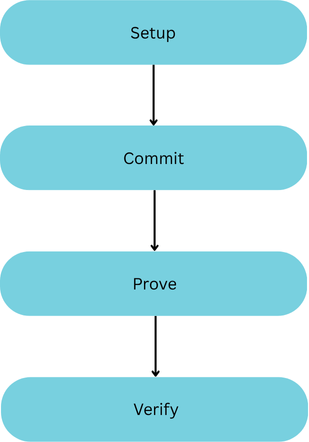
\includegraphics[width=0.4\textwidth]{BTP_ZKP Process.png}
\caption{Zero-Knowledge Proof Process}
\label{fig:zkp_process}
\end{figure}

\clearpage

% ============================================================================
% FIGURE 2: Theoretical Implementation
% ============================================================================
\section{Theoretical Implementation}

This implementation secures a pretrained logistic regression model by keeping its parameters $(w, b)$ confidential. When client inputs are provided as public data, the model generates predictions using the private parameters, and a zero-knowledge proof verifies the correctness of these predictions without revealing the weights or biases. Thus, clients can confirm that predictions are computed correctly using the claimed model while the model parameters remain fully private.

\begin{figure}[H]
\centering
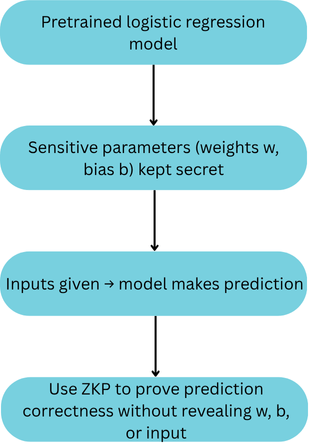
\includegraphics[width=0.4\textwidth]{BTP_Theoretical Implementation.png}
\caption{Theoretical Implementation of Zero-Knowledge Proof System}
\label{fig:theoretical_implementation}
\end{figure}

% ============================================================================
% FIGURE 3: Accuracy Verification Process
% ============================================================================
\section{Accuracy Proof Generation Process}

The Accuracy Proof Generation process begins with two inputs — the model’s claimed accuracy ($A_m$) and the client’s private dataset. The model is executed locally to compute the actual accuracy ($A_c$), and both values are compared inside an arithmetic circuit. If $A_m < A_c$, the system proceeds to generate a succinct SNARK proof certifying that the model’s accuracy claim is correct. The client then verifies this proof without accessing any private data, ensuring honest reporting and privacy-preserving evaluation.

\begin{figure}[H]
\centering
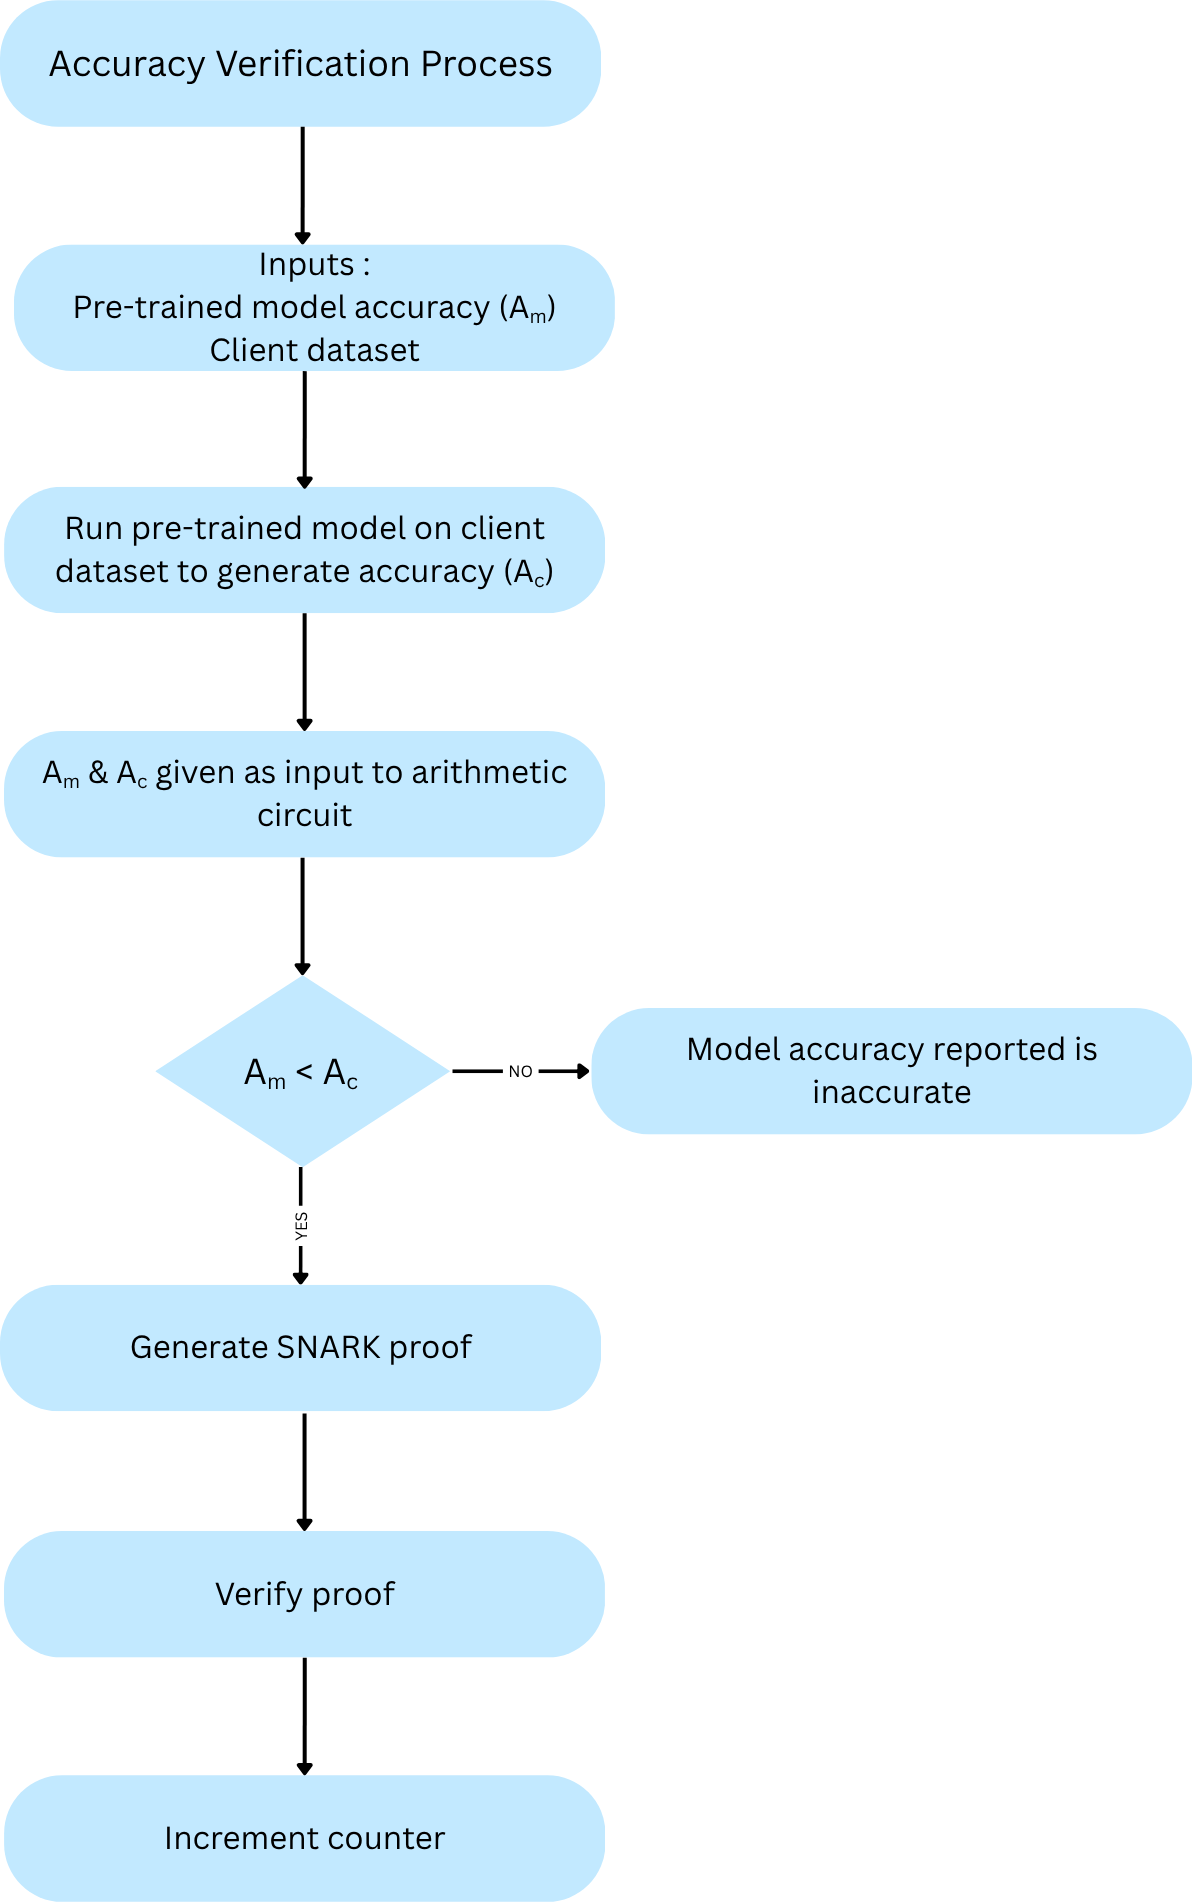
\includegraphics[width=0.6\textwidth]{BTP_Accuracy Proof Process.png}
\caption{Accuracy Verification Process}
\label{fig:accuracy_verification}
\end{figure}

% ============================================================================
% FIGURE 4: System Architecture
% ============================================================================
\section{System Architecture}

The architecture involves three entities: the Client (Verifier), Server (Prover), and a Trusted Third Party responsible for one-time setup. The system operates through a two-layer recursive SNARK framework. In the first layer, the server generates batch proofs for groups of samples, where each batch proof cryptographically verifies the correctness of individual predictions and counts the number of accurate predictions within that batch. In the second layer, an aggregator circuit recursively composes these batch proofs to verify that the total accuracy across all batches meets or exceeds the claimed threshold. The client receives a single compact final proof $\pi_{final}$ along with public inputs including the dataset hash, total sample count, and aggregate correct prediction count. By verifying this constant-size proof, the client can confirm the model's accuracy claim without learning individual predictions or model parameters, achieving scalable and privacy-preserving prediction and accuracy verification.

\begin{figure}[H]
\centering
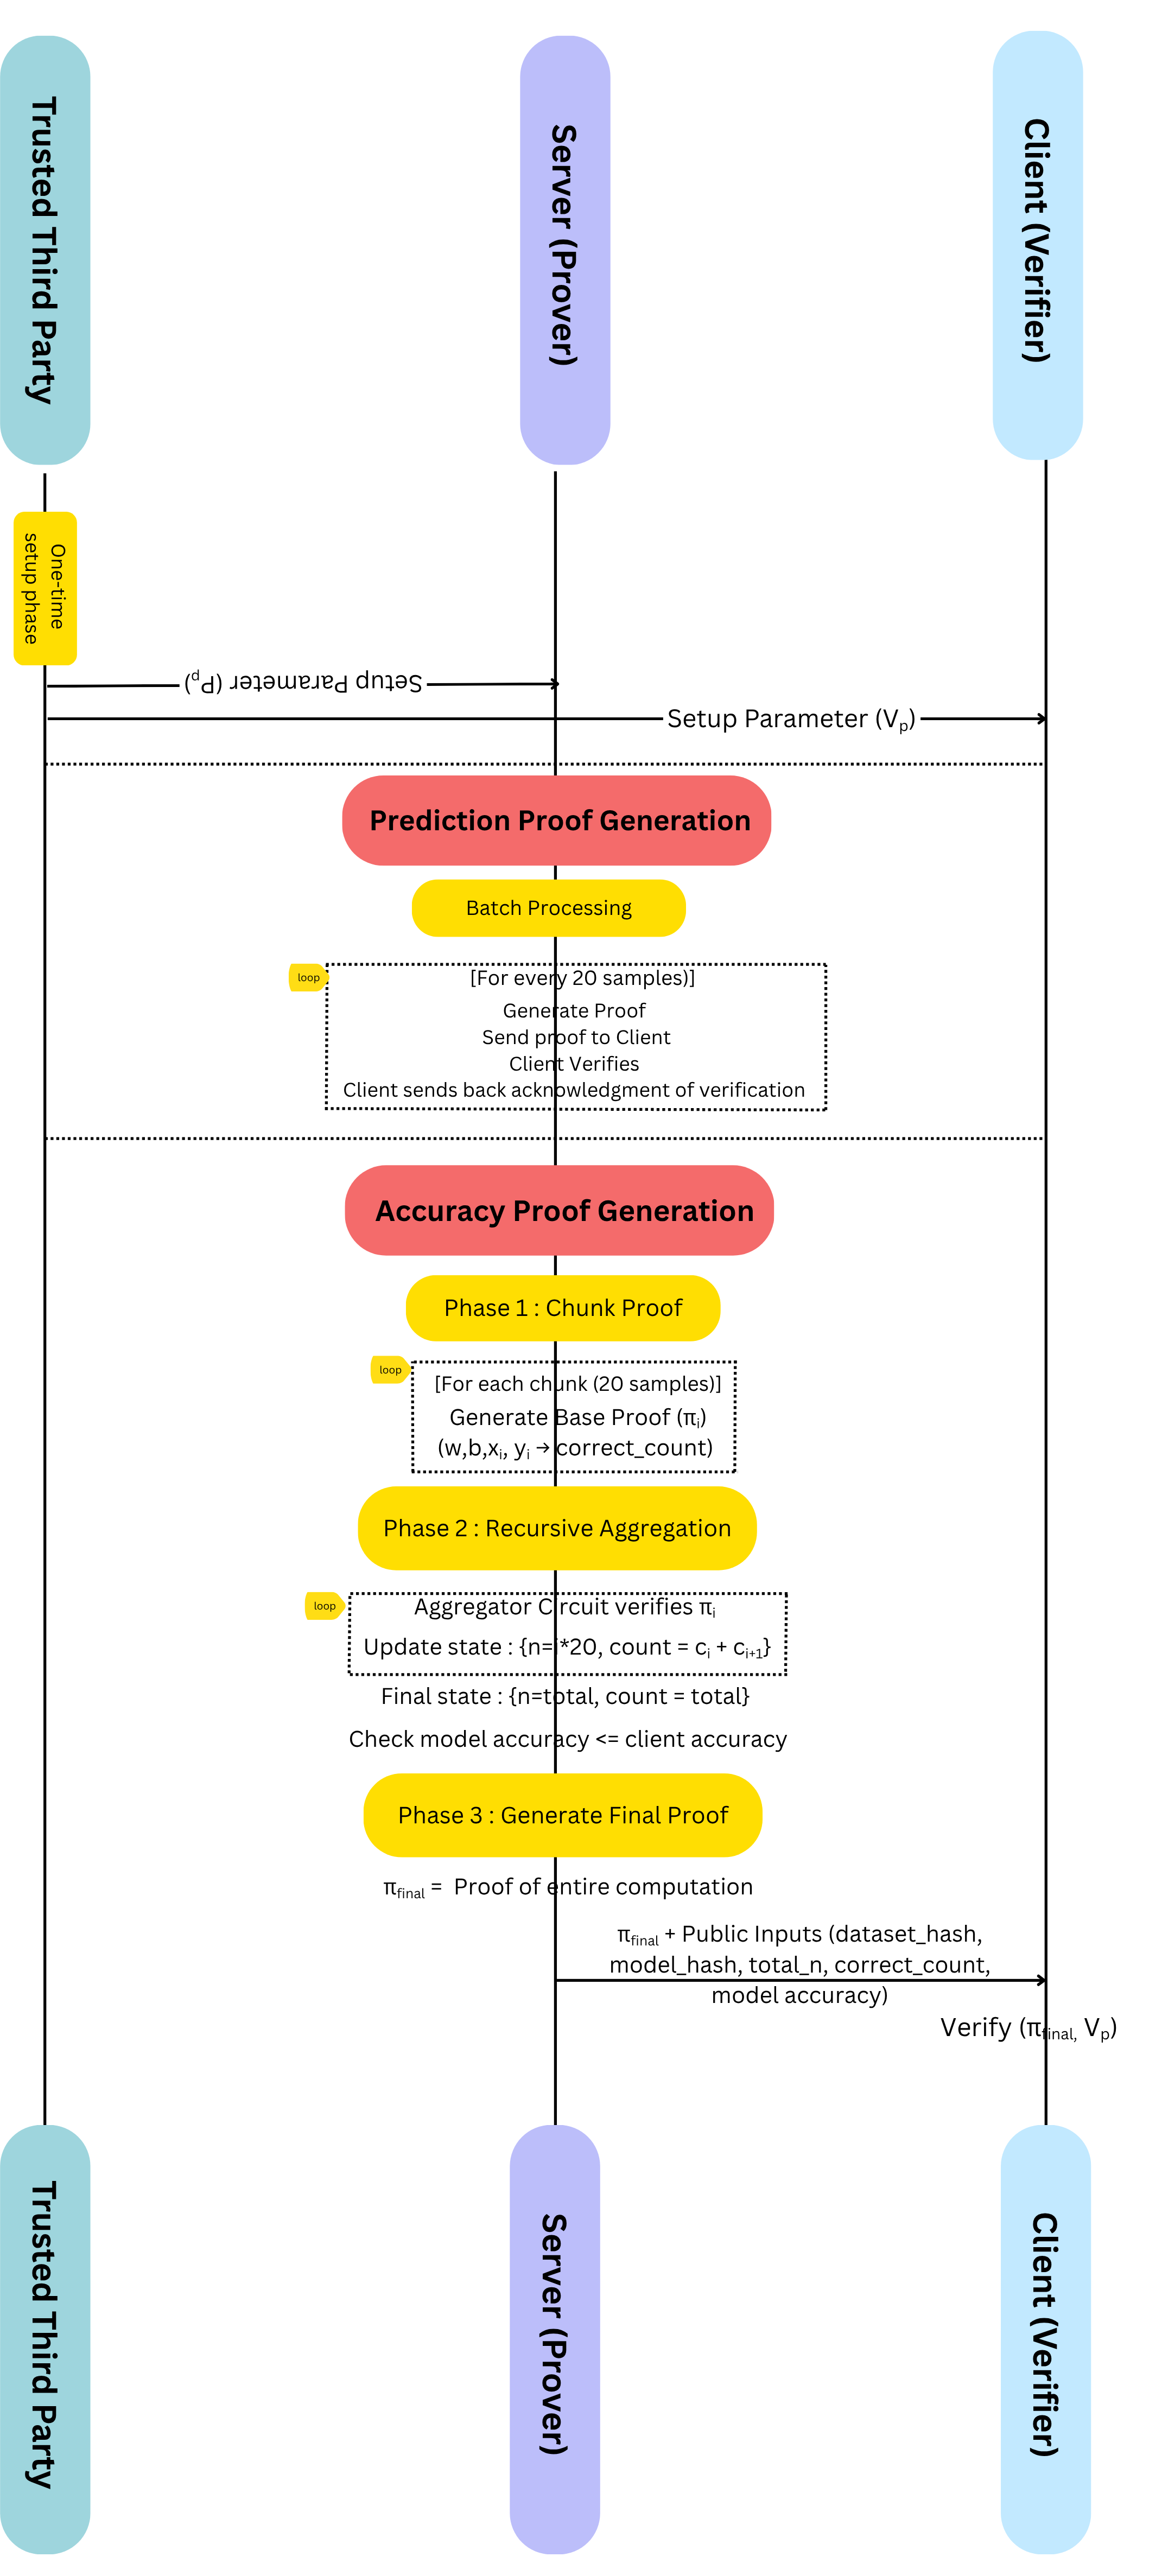
\includegraphics[width=0.565\textwidth]{sysarch.png}
\caption{System Architecture for Prediction Proof and Accuracy Proof generation}
\label{fig:system_architecture}
\end{figure}

\chapter{Detailed Implementation}
\label{chap:detailed-implementation}

This chapter summarizes the implementation details of the Zero-Knowledge Logistic Regression (ZKLR) system. The design integrates machine learning computation, zero-knowledge circuits, and cryptographic proof generation into a coherent workflow that demonstrates practical privacy-preserving inference. The implementation focuses on correctness, reproducibility, and computational efficiency while maintaining modularity for future extensions.

% =====================================================================
\section{System Architecture}
% =====================================================================

\subsection{Overview}

The ZKLR system adopts a modular architecture separating dataset preparation, model training, proof generation, verification, and performance evaluation. This design aligns with modern ZKP workflow practices that separate circuit compilation, witness generation, and proof verification. The data layer generates a synthetic dataset and trains a logistic regression model under controlled conditions. The proof-generation layer transforms inputs into witness assignments and constructs PLONK proofs demonstrating correct model inference without revealing private values, following the zero-knowledge definition introduced by Goldwasser et al.. Verification validates these proofs efficiently, and a metrics layer collects runtime statistics and visualizes performance behaviour.

\subsection{Technology Stack}

The implementation combines Python for numerical computation and Go for proof generation. Go 1.24.1 supports the gnark framework (v0.11.0), implementing PLONK-style proof systems as described by Kates et al.. Python 3.8+ facilitates dataset generation, logistic regression training, and plotting. The hybrid design leverages Python's machine learning ecosystem while ensuring performance and type safety during cryptographic operations.

% =====================================================================
\section{Dataset Handling}
% =====================================================================

\subsection{Dataset Overview}

A synthetic dataset containing 3,000 samples forms the evaluation baseline. Each record consists of a single numerical feature representing student marks from 0 to 100, accompanied by binary pass–fail labels. The reproducibility of the dataset is ensured through fixed random seeds, following standard practices in logistic regression modeling.

\subsection{Dataset Generation and Training}

The dataset is generated using uniform sampling followed by rule-based labeling, with added noise to prevent deterministic separation. Logistic regression is trained using scikit-learn with default parameters. The learned weights and bias are exported and encoded into fixed-point representations suitable for arithmetic circuits, bridging the floating-point domain with finite-field computation.

% =====================================================================
\section{Model Design}
% =====================================================================

\subsection{Logistic Regression Formulation}

Logistic regression estimates probabilities by evaluating the linear function
\begin{equation}
    z = wx + b
\end{equation}
and applying the sigmoid function
\begin{equation}
    \sigma(z) = \frac{1}{1 + e^{-z}},
\end{equation}
as defined in classical statistical modeling literature. The model’s simplicity and numerical stability make it suitable for zero-knowledge circuit construction, where each operation must be represented using finite-field arithmetic.

\subsection{Fixed-Point Encoding}

Since finite-field arithmetic does not natively support floating-point operations, values are encoded using fixed-point formats. In this representation, a value is stored as an integer scaled by a fixed power of two, where the format Qm denotes m fractional bits of precision. The system uses Q32 (32 fractional bits) for intermediate linear computations, Q10 (10 fractional bits) for indexing logits into the sigmoid lookup table, and Q16 (16 fractional bits) for final outputs. This multi-precision strategy balances accuracy and computational cost, ensuring numerical stability and preventing overflow, consistent with principles from ZKP arithmetic circuit design.

% =====================================================================
\section{Circuit Construction}
% =====================================================================

The circuit verifies that the predicted label corresponds to a valid logistic regression inference without revealing private model weights or intermediate values. Its structure ensures completeness, soundness, and zero-knowledge as established in.

\subsection{Circuit Configurations and System Parameters}

\begin{figure}[h]
    \centering
    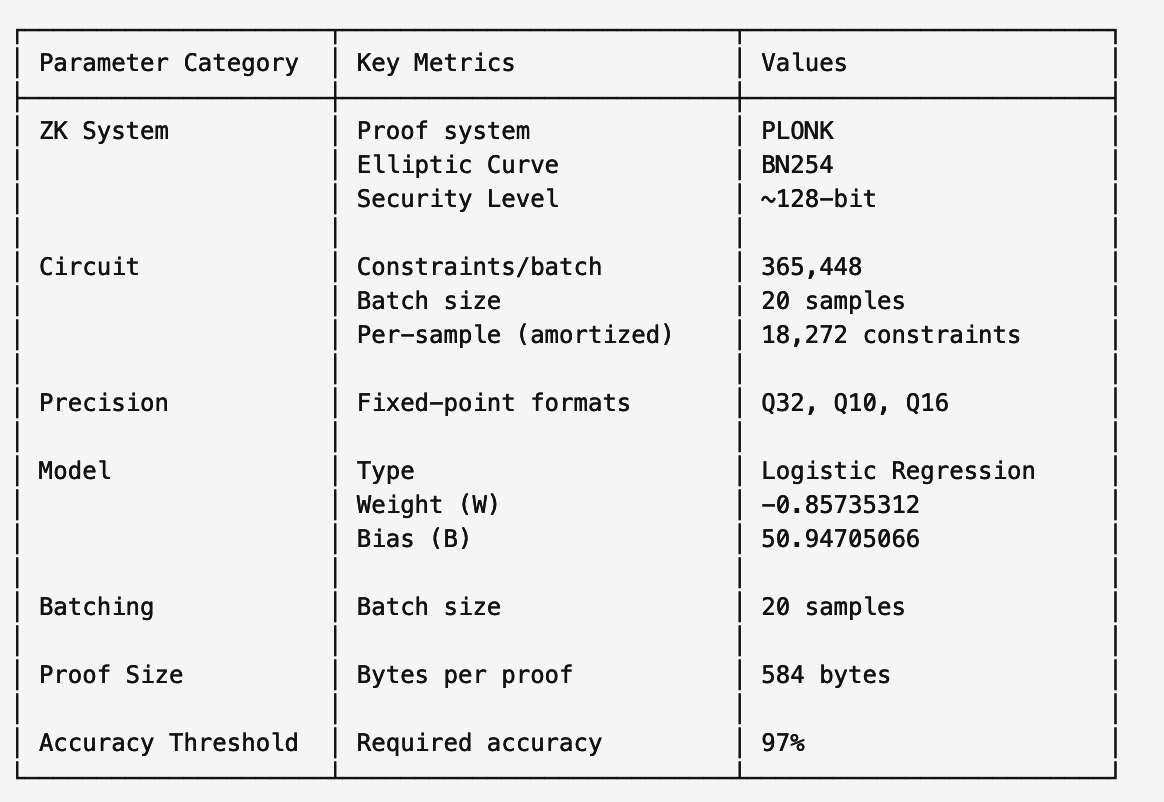
\includegraphics[width=0.75\textwidth]{congifs_invert.png}
    \caption{Configurations for the circuit}
    \label{fig:configuration}
\end{figure}

This image summarizes the core configuration parameters used in the zero-knowledge logistic regression system. These parameters define the circuit’s structure, numerical precision, proof characteristics, and batching strategy adopted during proof generation. The configuration reflects a trade-off between computational efficiency and verification soundness, ensuring both practical performance and strong cryptographic guarantees.

\subsection{Circuit Layers}

The sigmoid function is implemented using a lookup table of 8,192 precomputed values. This avoids evaluating exponentials inside the circuit, consistent with efficiency practices in ZKP systems. Symmetry is used to halve storage requirements via the identity 

\begin{equation}
    \sigma(-z) = 1 - \sigma(|z|),
\end{equation}

ensuring correctness within the finite-field framework. The final computation binds the predicted label to the claimed output, enforcing soundness.

\subsection{Circuit Algorithm}
The circuit algorithm defines the constraints required to verify logistic regression inference within the zero-knowledge framework. It encodes both the linear computation and the non-linear sigmoid transformation as arithmetic operations over a finite field.

\begin{figure}[h]
    \centering
    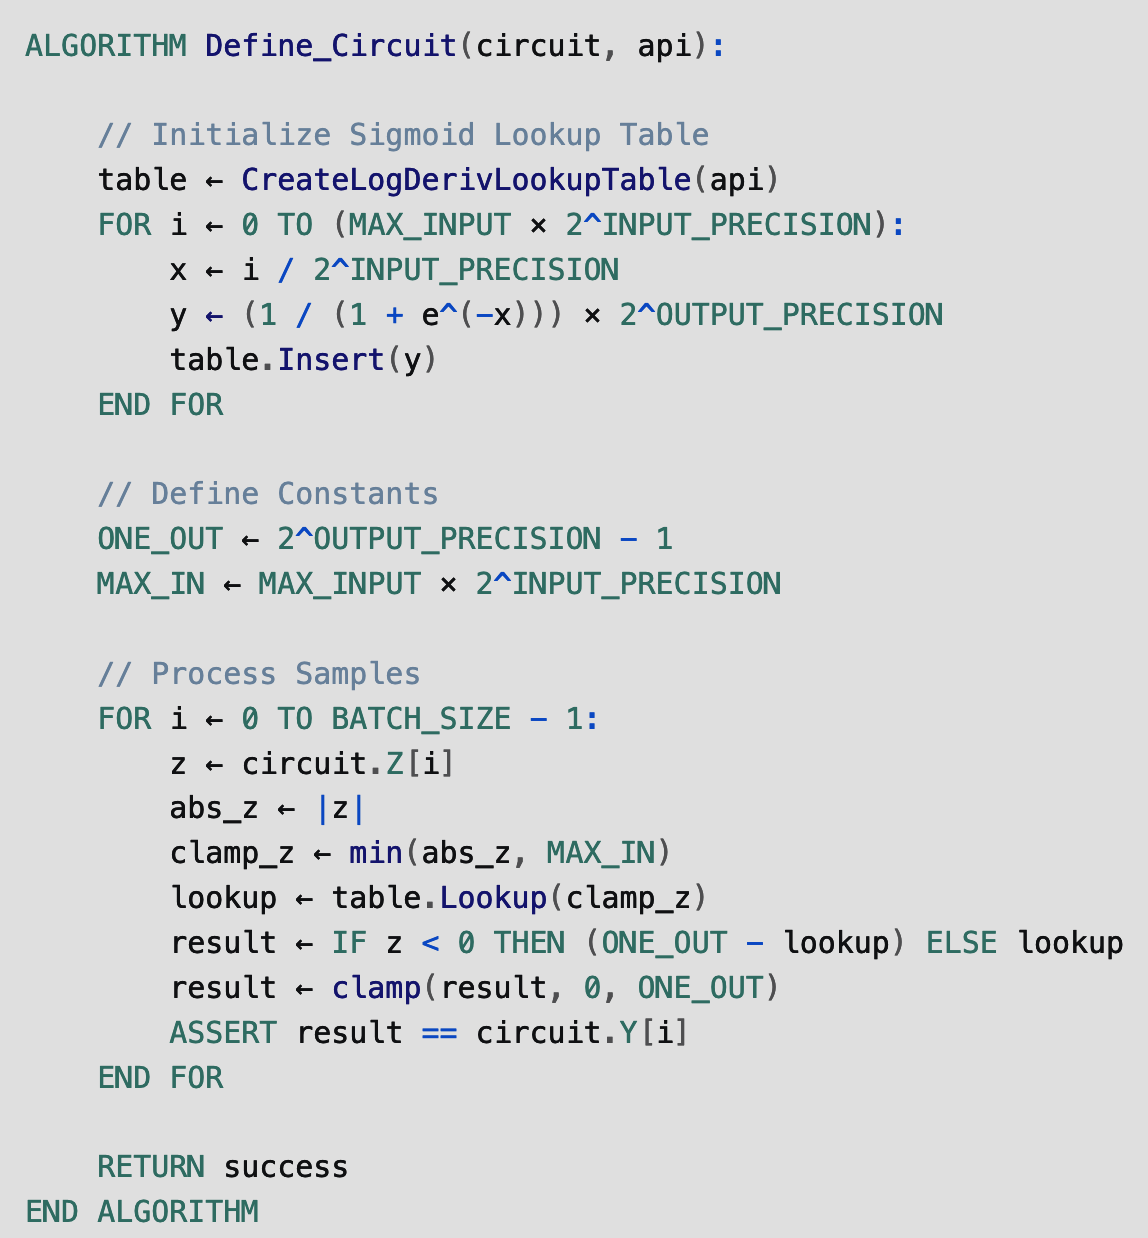
\includegraphics[width=0.75\textwidth]{image (2).png}
    \caption{Pseudocode for Circuit Algorithm}
    \label{fig:algorithm}
\end{figure}

This algorithm captures the full inference pipeline of logistic regression within an arithmetic circuit. By representing each operation as a verifiable constraint, it ensures that the prover can only produce valid proofs corresponding to genuine model computations, thus preserving soundness and correctness under zero-knowledge guarantees.

\subsection{Constraint Count}

The optimized circuit contains 58,028 constraints. Lookup-table enforcement forms the majority of these constraints, reflecting the complexity inherent in embedding non-linear functions into arithmetic circuits. Remaining constraints ensure correctness of sign handling, linear computation, and output binding.

\subsection{Constraint Design}
The arithmetic circuit enforces the correctness of the logistic regression inference through a layered set of constraints. Each constraint corresponds to a verifiable algebraic relationship that ensures the model’s output is consistent with the claimed computation.

\begin{figure}[H]
    \centering
    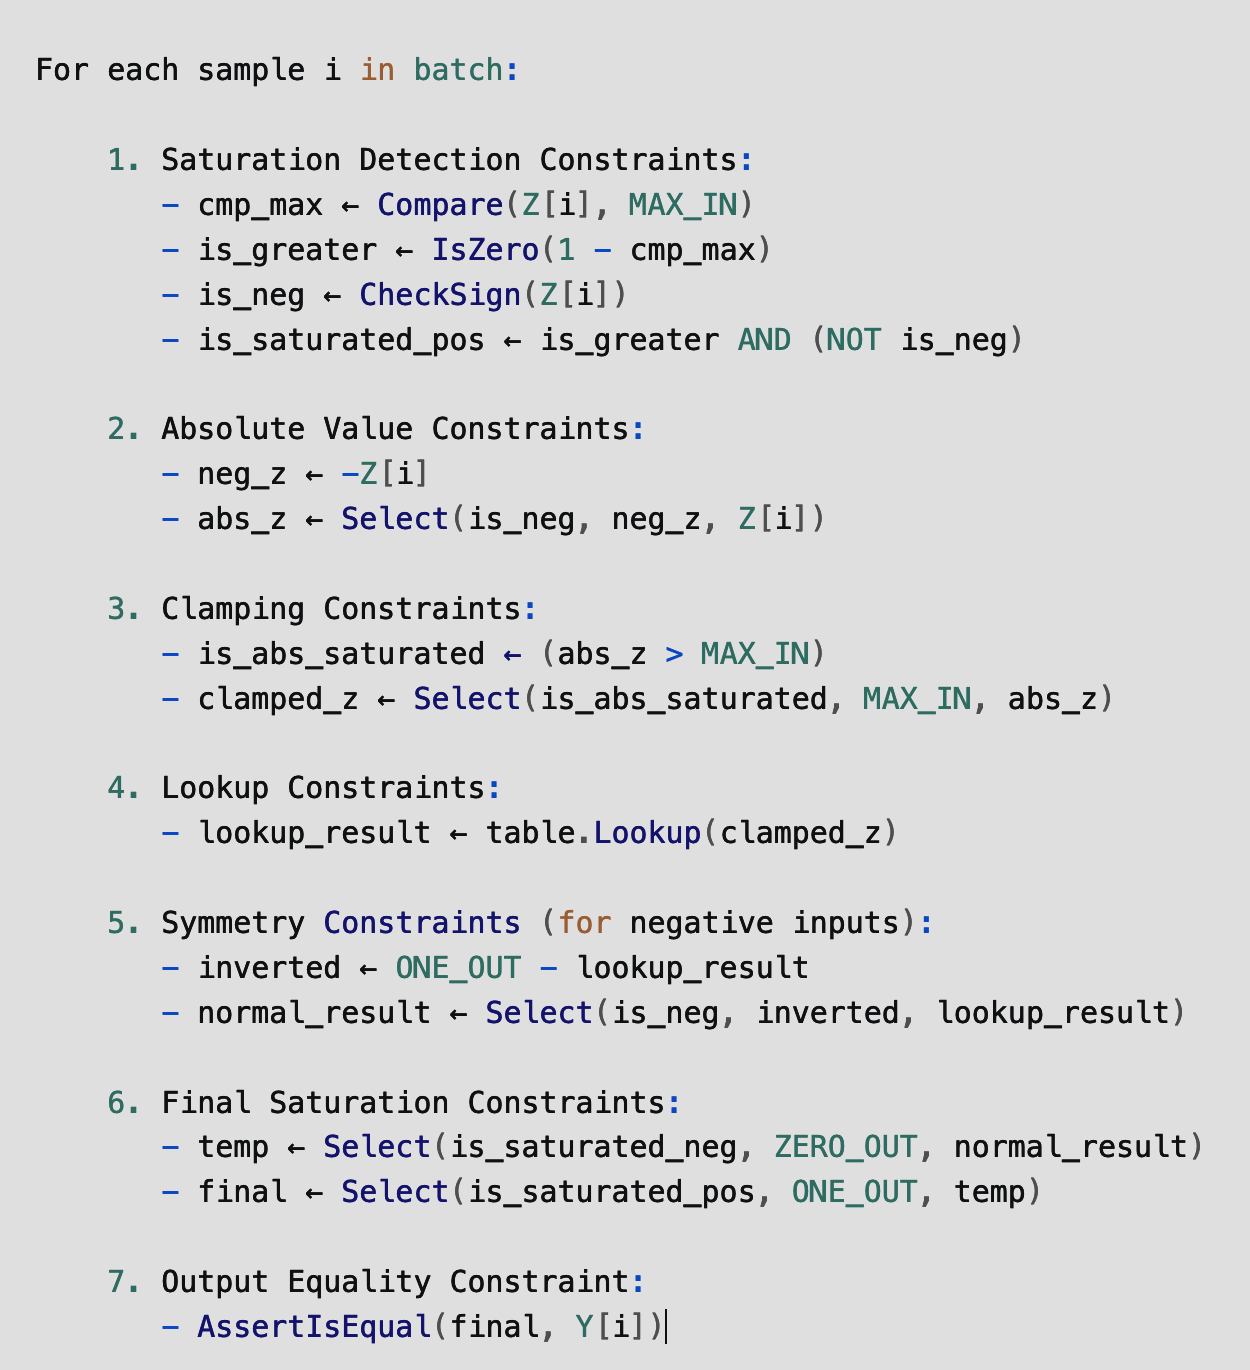
\includegraphics[width=0.75\textwidth]{constraints.png}
    \caption{Constraints in Arithmetic Circuits}
    \label{fig:constraints}
\end{figure}

Together, these constraints ensure that the circuit remains sound, complete, and consistent with the logistic regression inference function, while adhering to the zero-knowledge property.

% =====================================================================
\section{Proof Generation Workflow}
% =====================================================================

\subsection{Setup Phase}

Proof generation starts with compiling the circuit  and generating keys for the prover and verifier using the PLONK protocol. This setup step is performed once per circuit and remains constant regardless of dataset size.

\begin{figure}[h]
    \centering
    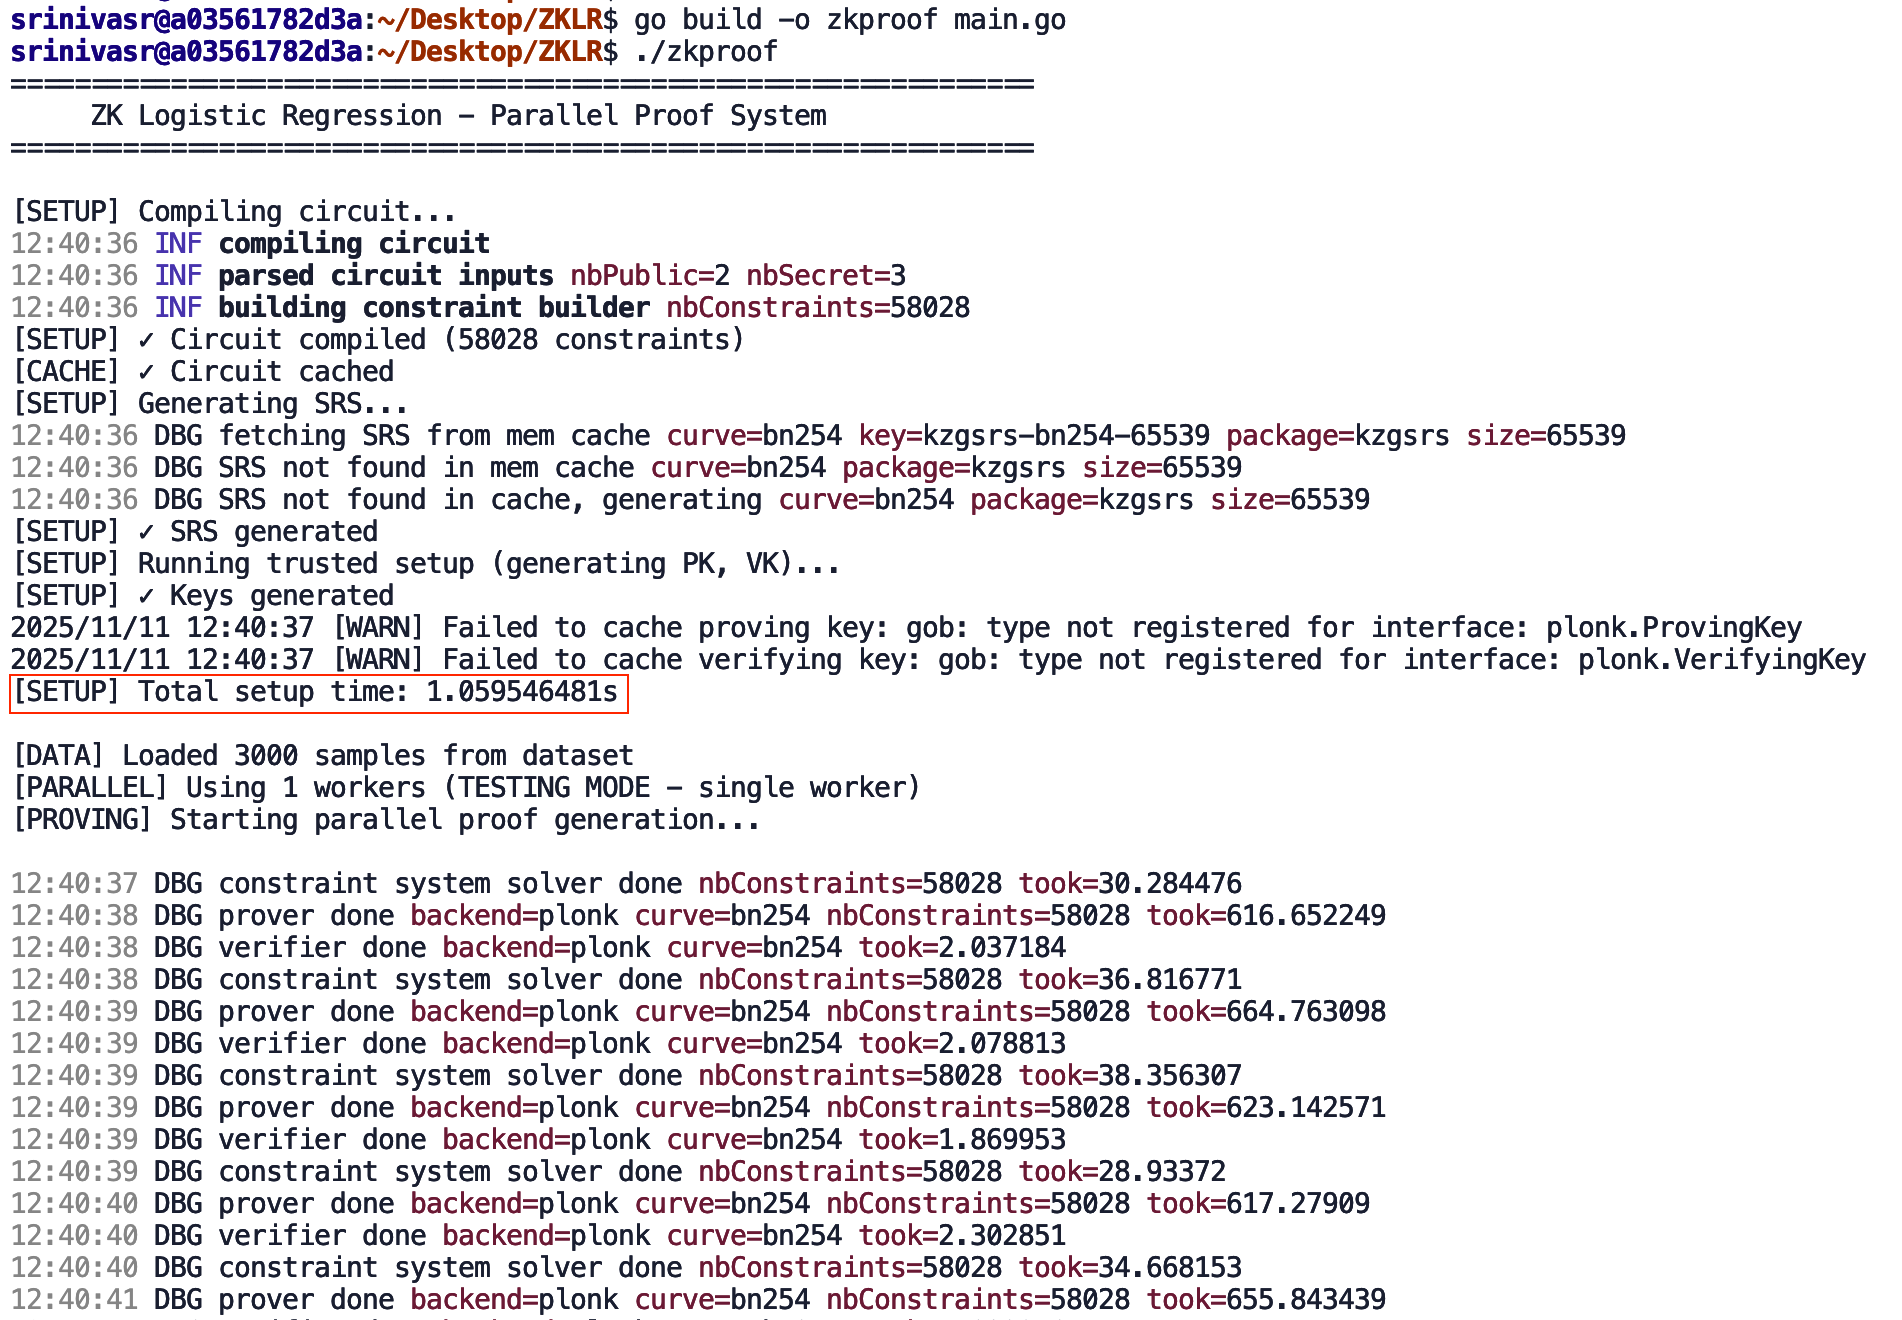
\includegraphics[width=0.75\textwidth]{image.png}
    \caption{Setup time for a circuit}
    \label{fig:setup_time}
\end{figure}

\subsection{Individual Proof Generation}

For each input sample, the system computes the linear score and sigmoid output using fixed-point arithmetic. These values populate the private witness required for proof generation. The size of each PLONK proof is 584 bytes which is in line with the succinctness guarantee of the polynomial commitment scheme.

\begin{figure}[h]
    \centering
    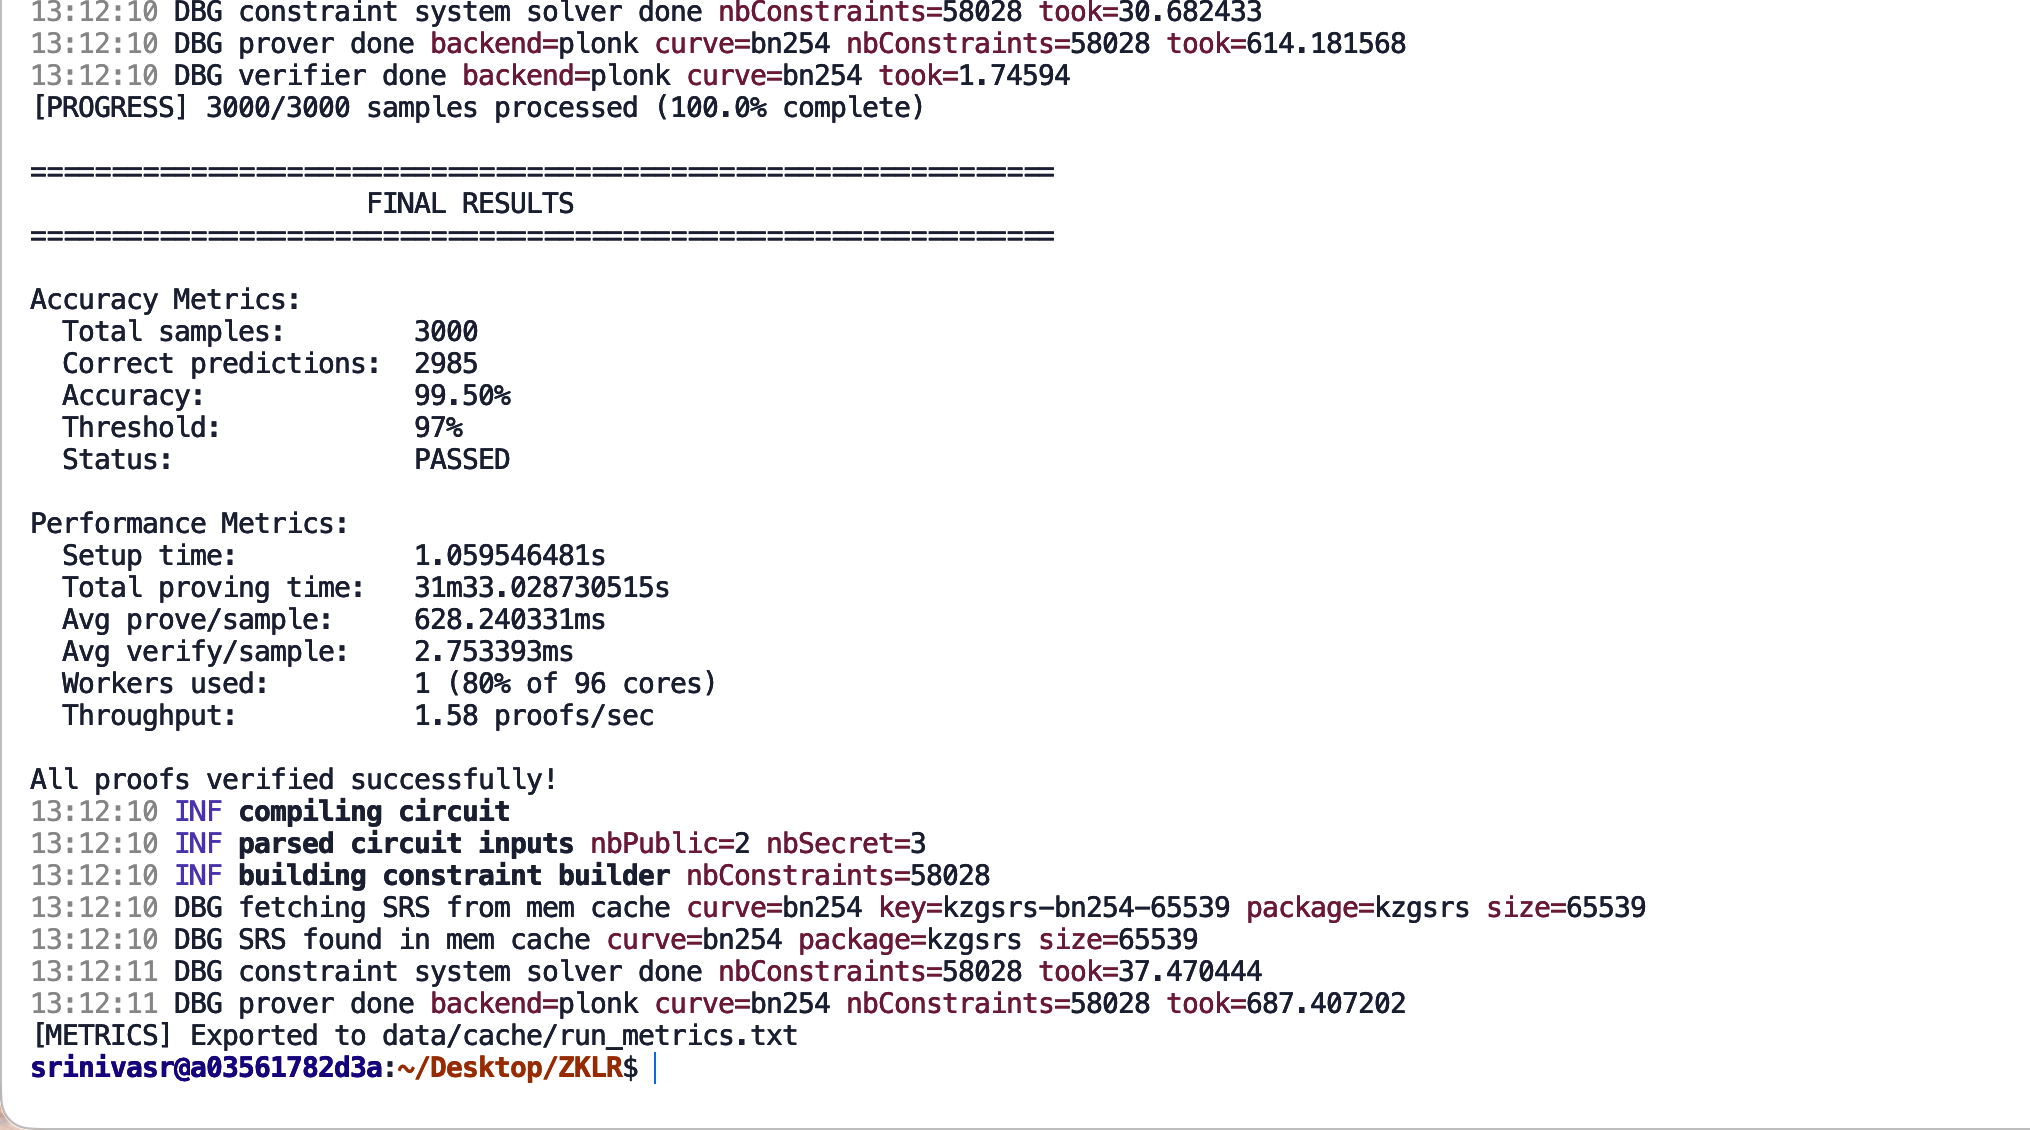
\includegraphics[width=0.75\textwidth]{3.png}
    \caption{Proof generation and verification for individual samples}
    \label{fig:sample_proof_time}
\end{figure}

Verifier validates the proof using the verification key and public inputs only, ensuring zero-knowledge properties as originally defined.

\subsection{Batched Proof Implementation}

Batch proving allows proofs to be generated for multiple samples within a single circuit instance. With 20 samples per batch, the circuit grows to 365,448 constraints but achieves sublinear scaling by reusing setup and lookup-table loading across samples.

\begin{figure}[H]
    \centering
    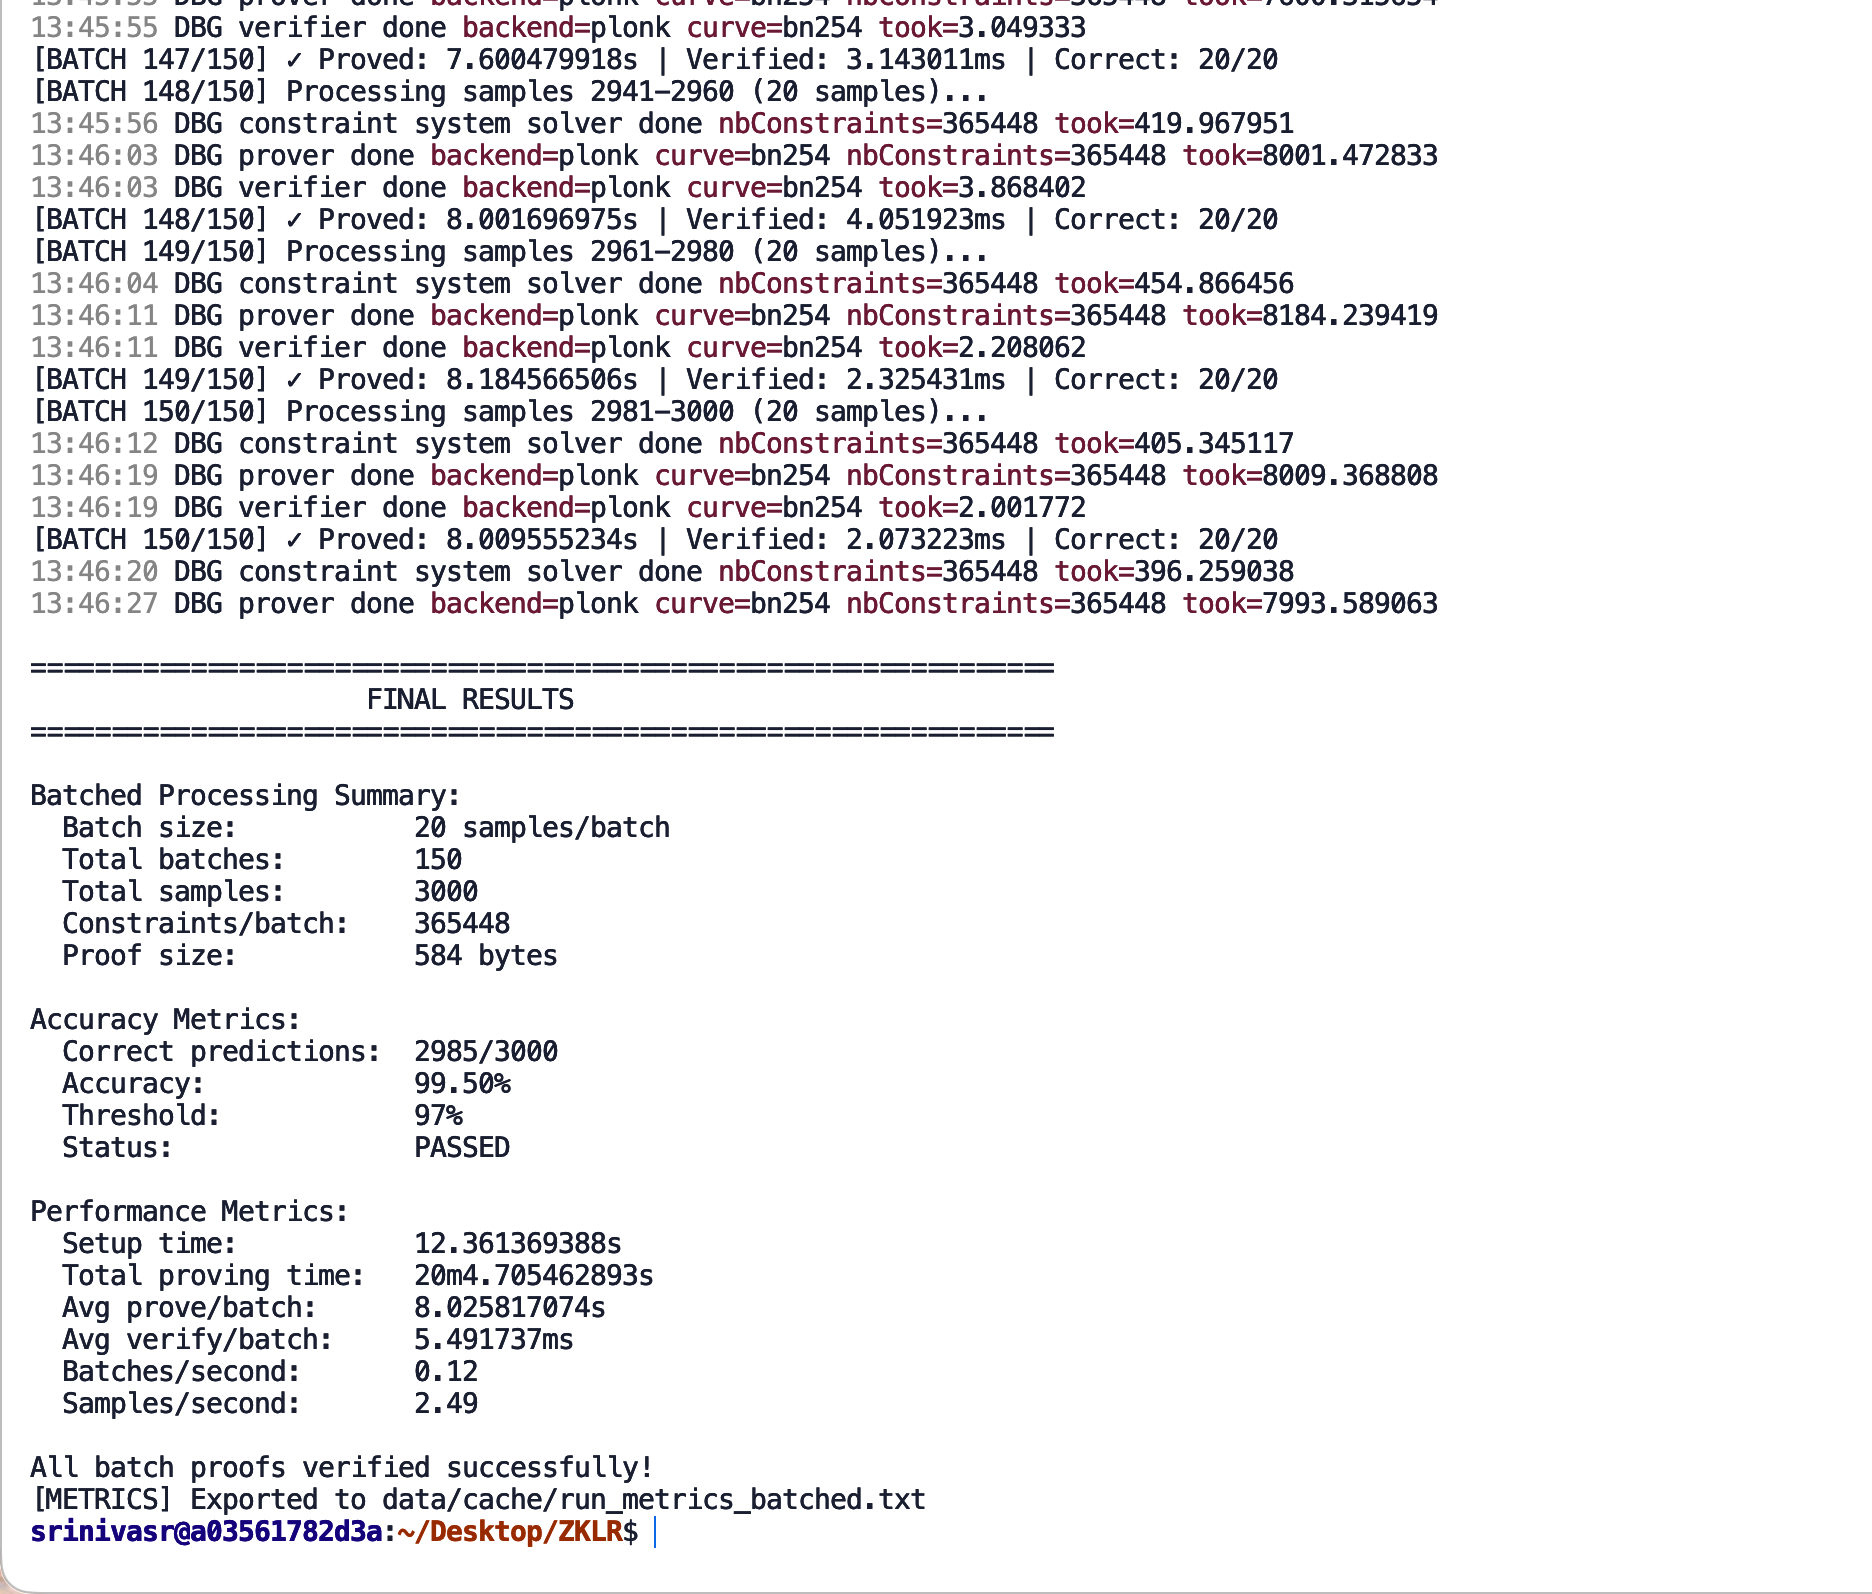
\includegraphics[width=0.75\textwidth]{5.png}
    \caption{Evaluation Metrics for Batched Proofs}
    \label{fig:batched_proof_time}
\end{figure}

% =====================================================================
\section{Performance Optimizations}
% =====================================================================

\subsection{Lookup Table Reduction}

Empirical analysis showed that logits predominantly fall within $[-8,8]$. Restricting the lookup table to this domain reduces entries from 30,720 to 8,192 thus lowering the constraint count and improving proving time by approximately 4.4 times.

\begin{figure}[H]
    \centering
    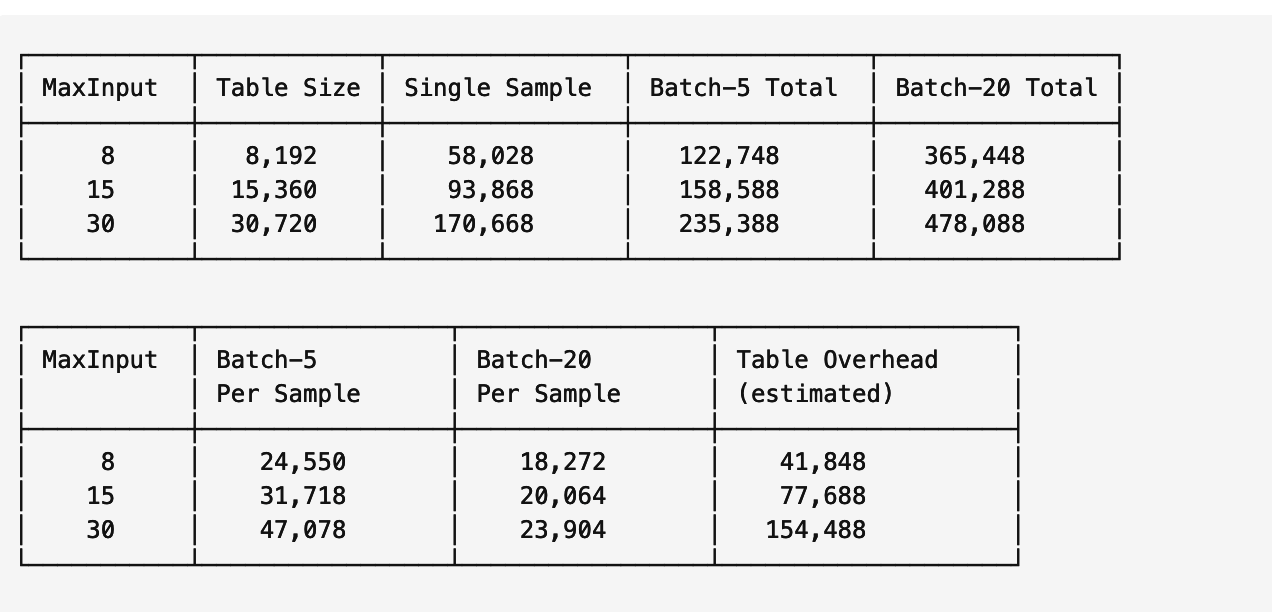
\includegraphics[width=0.75\textwidth]{image (3).png}
    \caption{Lookup Table for Non-linear function}
    \label{fig:lookup_table}
\end{figure}

\subsection{Circuit Caching and Precision Control}

Caching compiled circuits helps avoid repeated preprocessing. Controlled precision preserves numerical stability while minimizing constraint usage, aligning with modern practices in efficient ZK circuit optimization.

% =====================================================================
\section{Security Considerations}
% =====================================================================

The PLONK protocol provides zero-knowledge guarantees consistent with the foundational definition. Soundness relies on the hardness of the discrete logarithm problem over the BN254 elliptic curve, offering approximately 128-bit security. Although this prototype uses a single-party structured reference string (SRS), production environments require multi-party ceremonies to prevent toxic waste retention.

% =====================================================================
\section{Summary}
% =====================================================================

The implementation demonstrates feasible and efficient zero-knowledge verification of logistic regression. The architecture integrates machine learning computation with fixed-point encoding, lookup-table optimization, and cryptographic proof generation. This design ensures strong privacy, predictable runtime behaviour, and accurate classification results, forming a robust foundation for future exploration of zero-knowledge machine learning frameworks.

\chapter{Results and Observations}

This chapter presents the experimental results obtained from implementing Zero-Knowledge Logistic Regression using the GNARK framework. Analysis was done for proof sizes, performance, scalability, batch processing efficiency, and security validation. All experiments were conducted on a fixed dataset of 500 student records with varying batch sizes ranging from 5 to 100 samples per proof to determine the optimal batching strategy.

\section{Proof Size Analysis}

The PLONK proof system demonstrates constant proof size regardless of the circuit complexity or number of samples processed. 

\begin{figure}[h]
    \centering
    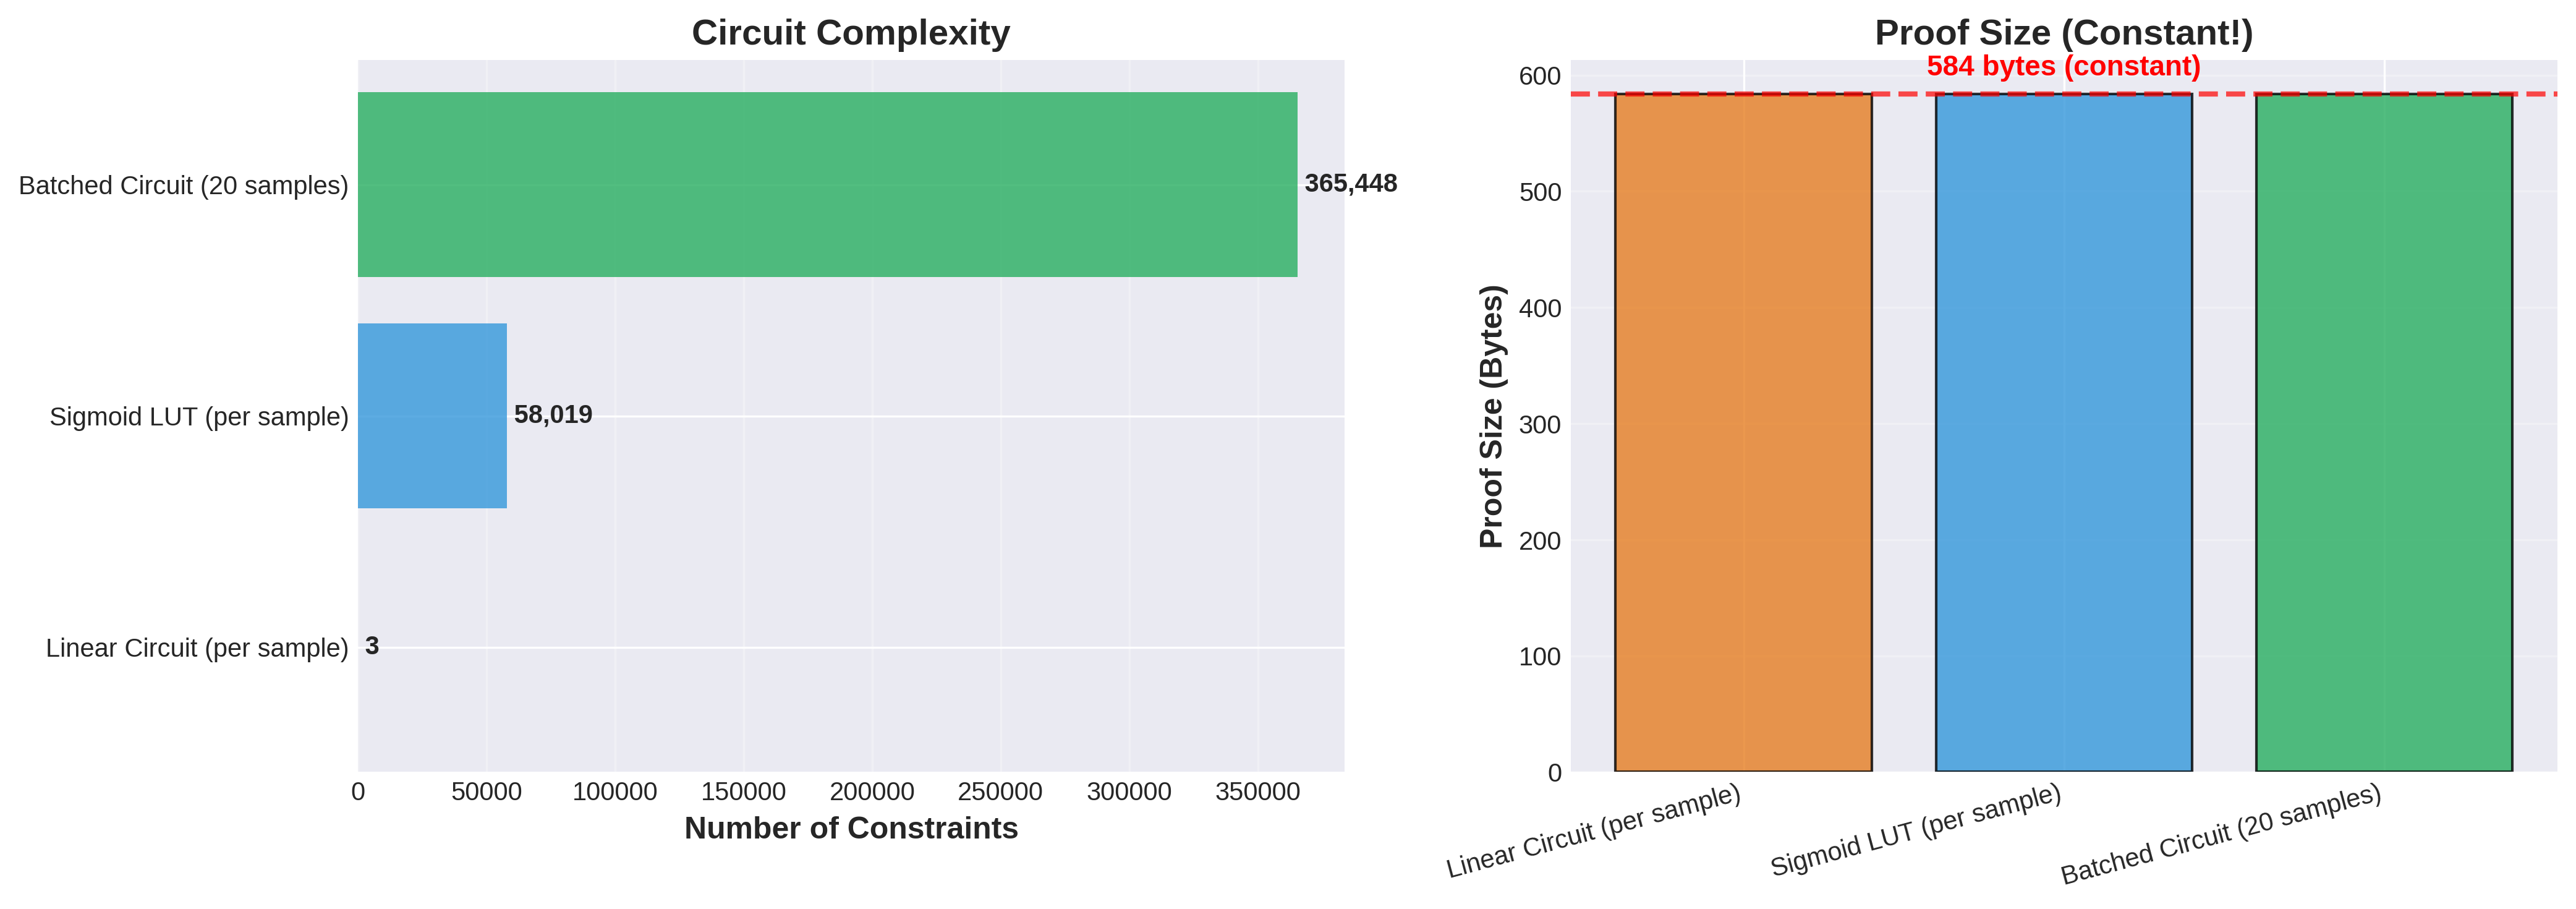
\includegraphics[width=0.8\textwidth]{proof_size_comparison.png}
    \caption{Constant proof size confirms succinctness of PLONK}
    \label{fig:proof_size_comparison}
\end{figure}

As shown in Figure~\ref{fig:proof_size_comparison}, both circuit implementations, individual samples and batched samples, generate proofs of exactly 584 bytes. The circuit for individual samples contains 58,028 constraints, whereas the batched version contains 365,448 constraints, yet both produce proofs of identical size. This constant proof size confirms PLONK's succinctness property, where the proof size depends only on the security parameter and not on the circuit complexity. The communication cost therefore remains minimal, regardless of the computation complexity being verified.

\section{Batch Size Optimization Analysis}

The selection of optimal batch size requires careful analysis of the trade-off between circuit complexity and proof generation overhead. Experiments were conducted with batch sizes of 5, 10, 20, 25, 50, and 100 samples per proof on a fixed dataset of 500 samples.

\begin{figure}[h]
    \centering
    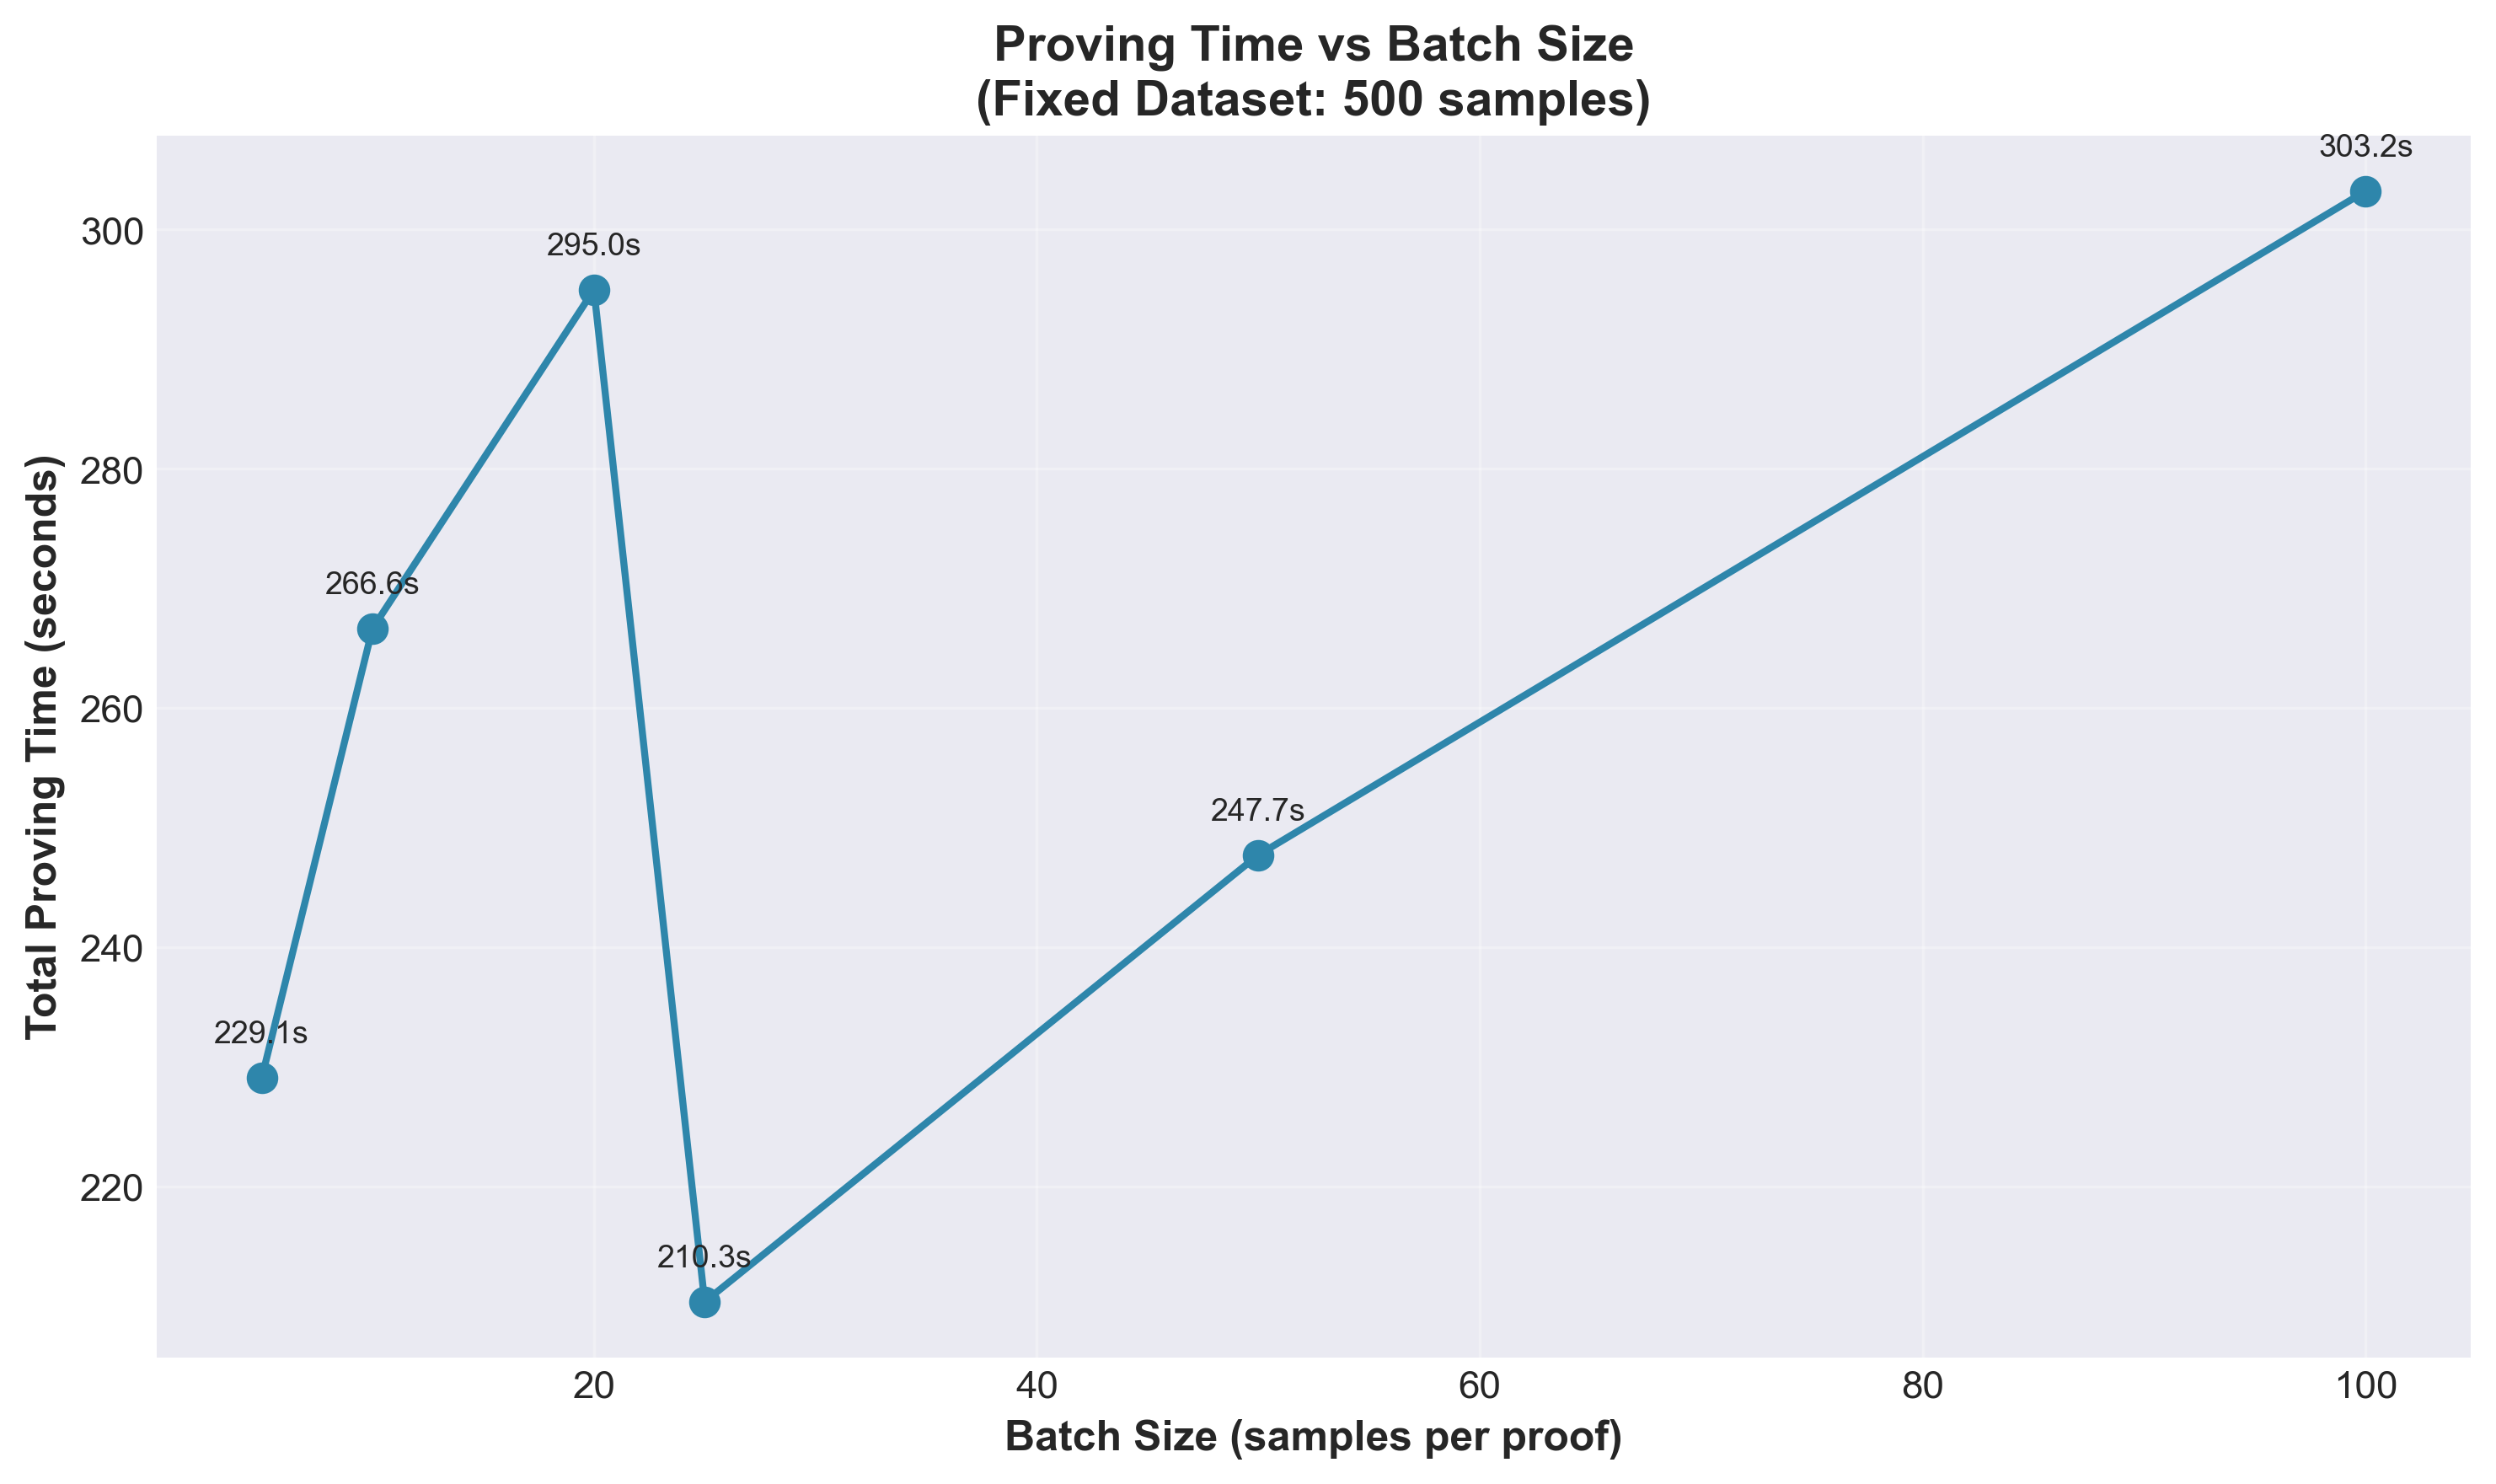
\includegraphics[width=0.8\textwidth]{batch_proving_time.png}
    \caption{Total proving time exhibits non-monotonic behavior across batch sizes}
    \label{fig:batch_proving_time}
\end{figure}

Figure~\ref{fig:batch_proving_time} reveals a critical finding that challenges the intuition that larger batches always improve performance. The proving time initially increases from 229 seconds at batch size 5 to a peak of 295 seconds at batch size 10, then drops sharply to 210 seconds at batch size 25 before rising again to 303 seconds at batch size 100. This non-monotonic behavior indicates that batch size 25 represents a local optimum where the circuit compilation and constraint satisfaction mechanisms achieve maximum efficiency. The sharp increase from batch size 5 to 10 suggests that small batches incur disproportionate overhead in circuit setup, while the subsequent decrease to batch size 25 demonstrates improved amortization of shared computation. Beyond batch size 25, the proving time increases linearly as circuit complexity dominates, with each additional sample contributing proportionally more constraints that offset the benefits of batching.

\section{Throughput Characteristics}

System throughput measures the rate at which samples can be processed, proved and verified, accounting for both proving and verification overhead.

\begin{figure}[h]
    \centering
    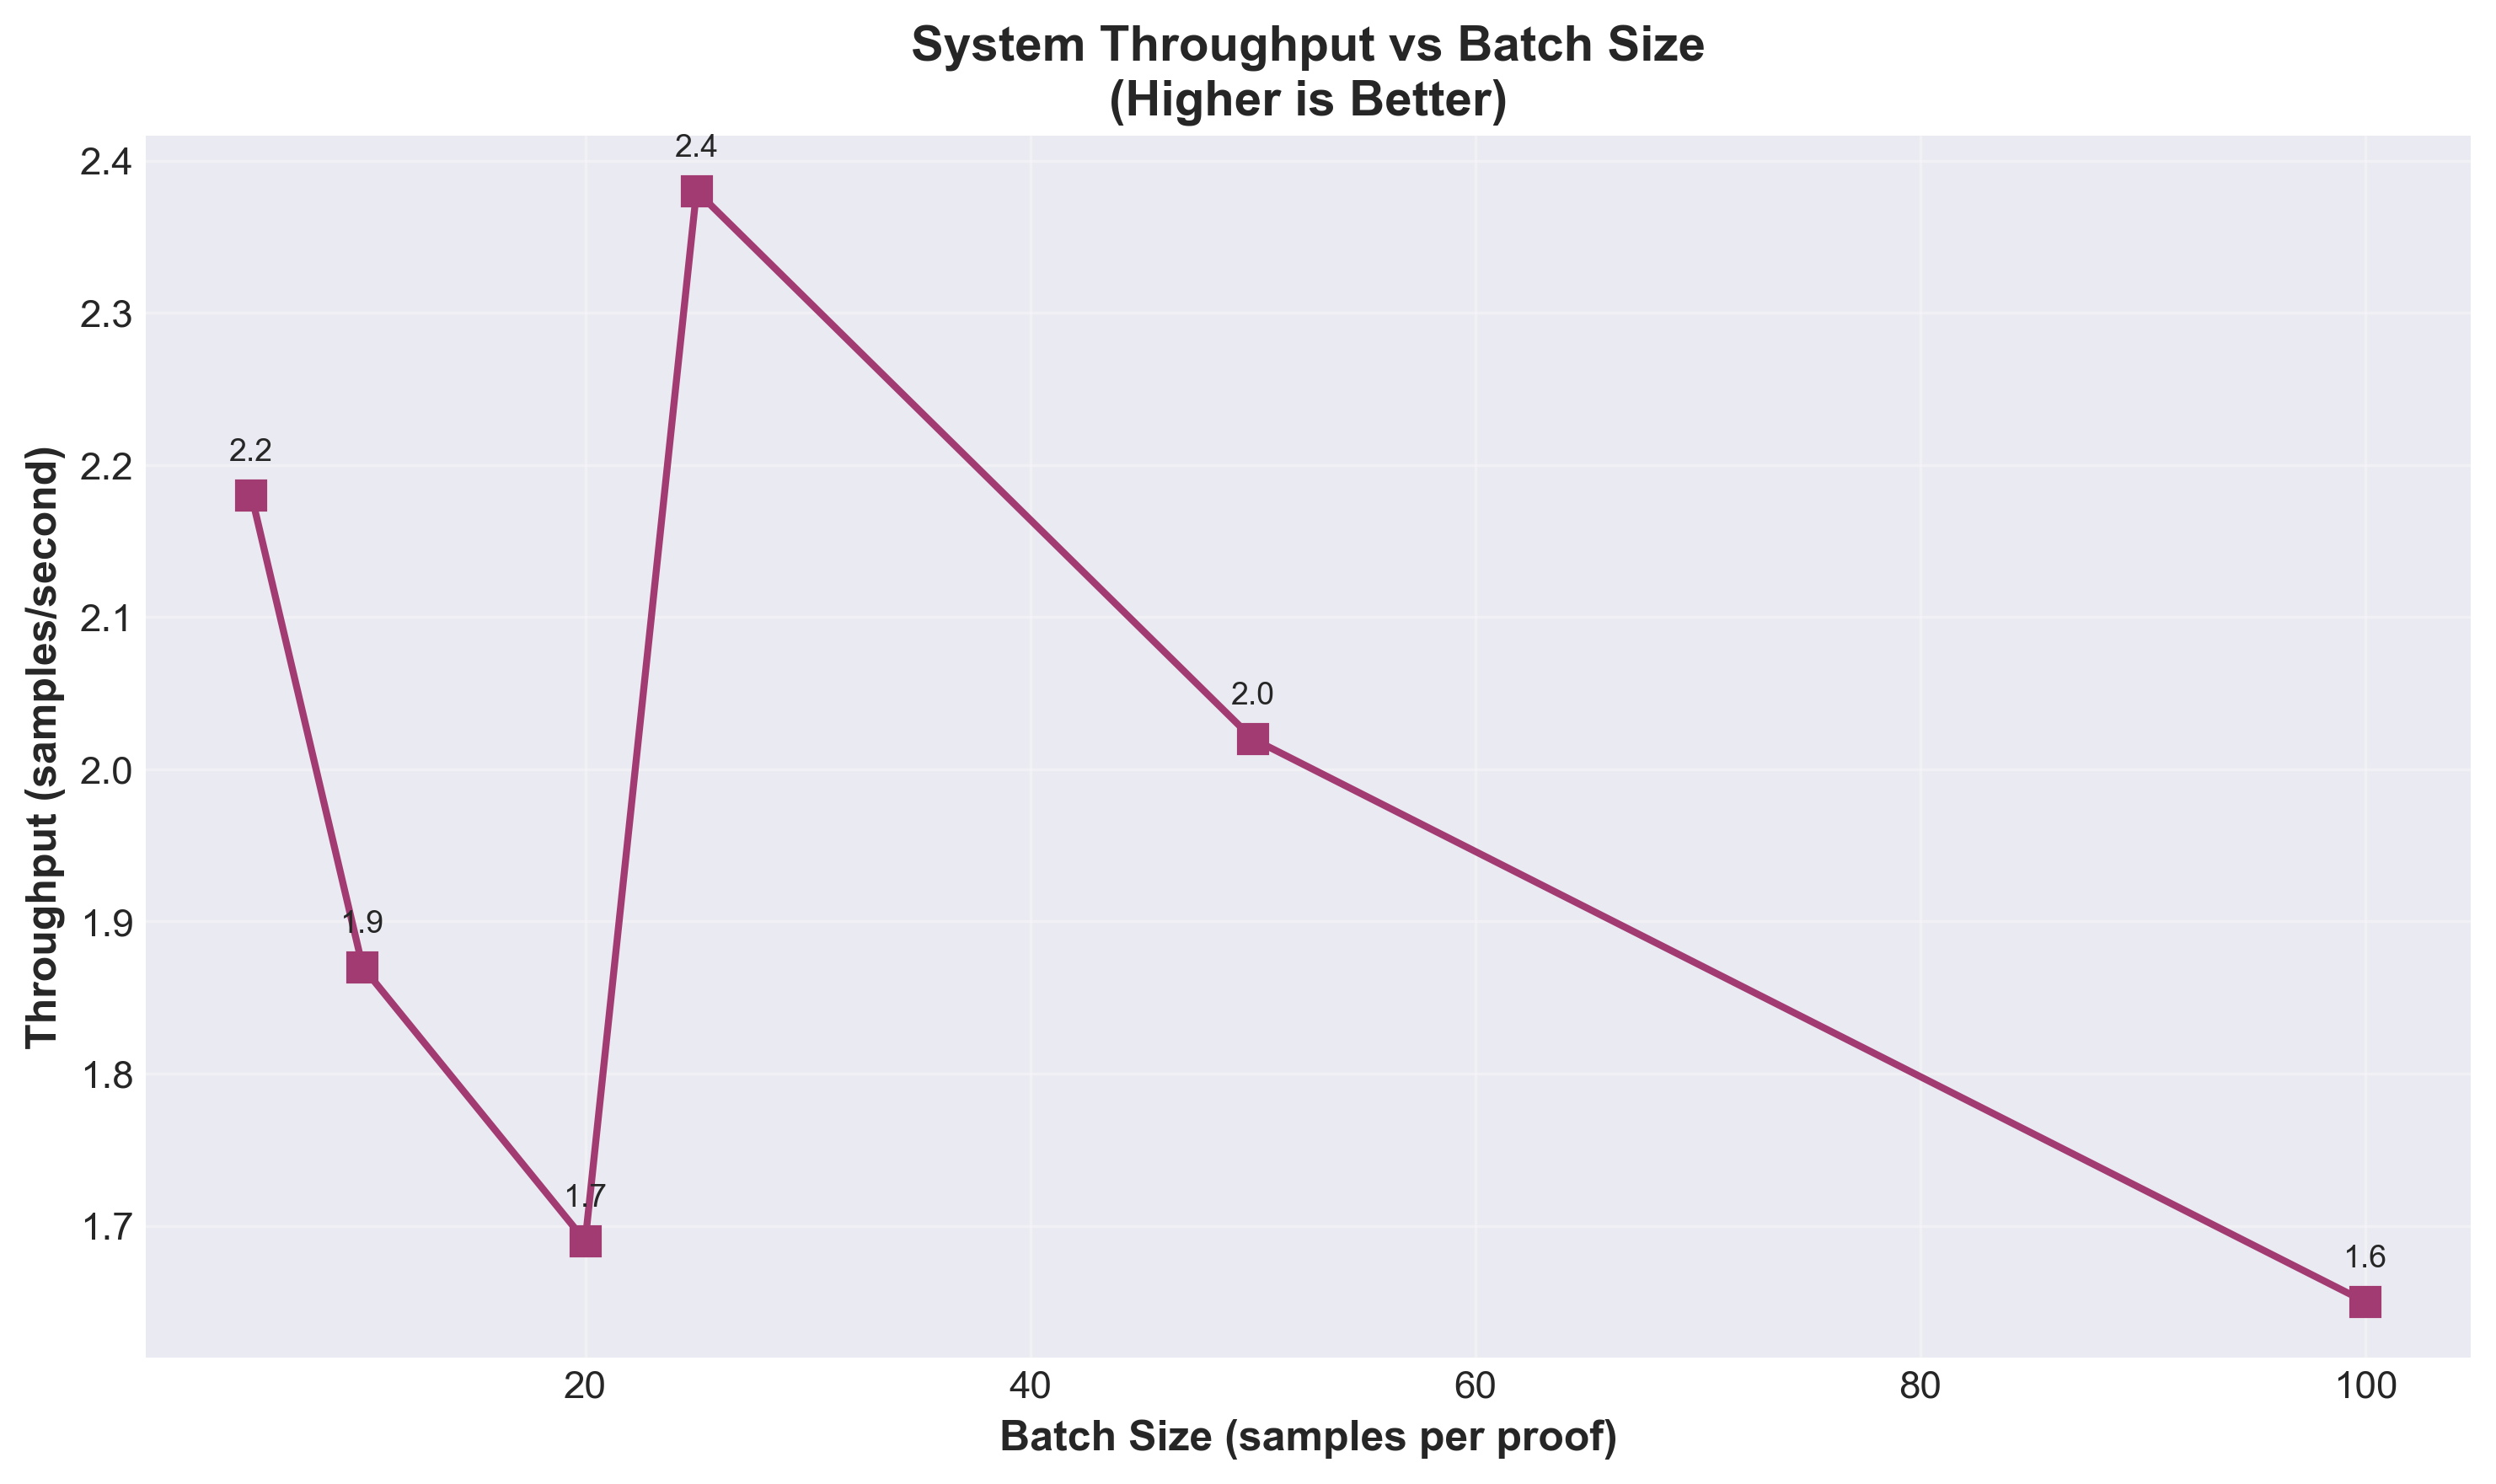
\includegraphics[width=0.8\textwidth]{batch_throughput.png}
    \caption{Throughput analysis reveals batch size 20 as the optimal configuration}
    \label{fig:batch_throughput}
\end{figure}

Figure~\ref{fig:batch_throughput} demonstrates that batch size 20 achieves the maximum throughput of 2.4 samples per second, processing the complete 500-sample dataset most efficiently. Smaller batch sizes of 5 and 10 achieve throughputs of 2.2 and 1.7 samples per second respectively, hampered by the overhead of generating more proofs with 100 and 50 proofs required respectively. Batch size 25 maintains competitive throughput at 2.4 samples per second due to its minimal proving time, while larger batch sizes of 50 and 100 experience degraded throughput of 2.0 and 1.6 samples per second as circuit complexity increases. The convergence of batch sizes 20 and 25 at peak throughput suggests a narrow optimal range where the balance between proof count reduction and circuit complexity is achieved. This finding indicates that deployment configurations should target batch sizes between 20 and 25 to maximize system efficiency, with batch size 20 preferred for slightly better throughput and batch size 25 preferred for minimal proving time.

\section{Circuit Complexity Analysis}

The growth of circuit constraints with batch size directly impacts both proving time and memory requirements.

\begin{figure}[h]
    \centering
    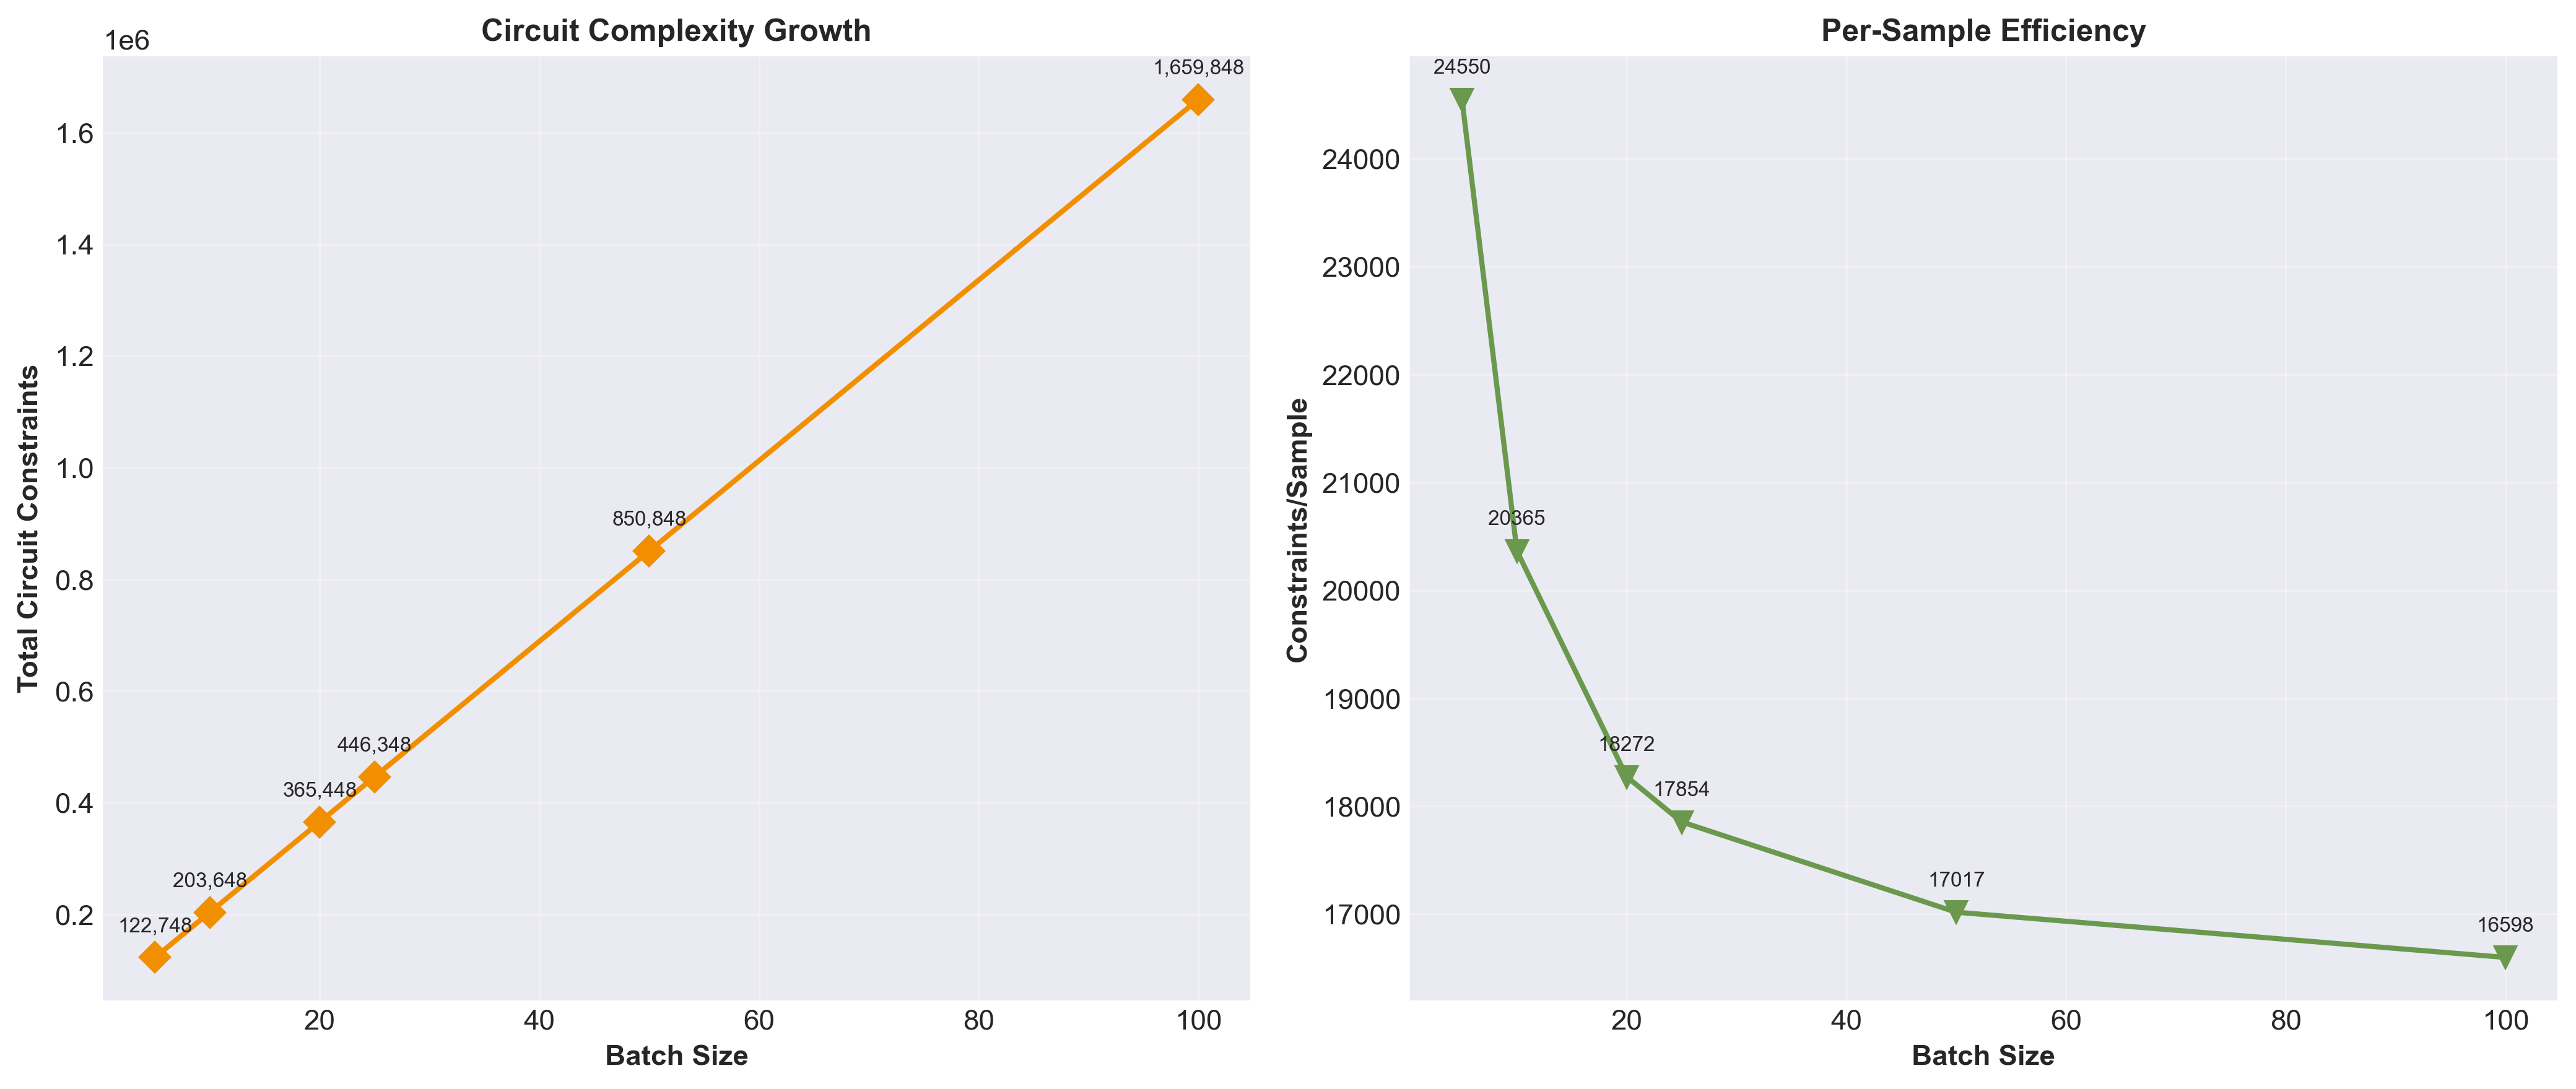
\includegraphics[width=0.8\textwidth]{batch_constraints.png}
    \caption{Circuit complexity grows linearly while per-sample efficiency improves}
    \label{fig:batch_constraints}
\end{figure}

Figure~\ref{fig:batch_constraints} illustrates the dual perspective on circuit complexity. The left panel shows total circuit constraints increasing linearly from 122,748 at batch size 5 to 1,659,848 at batch size 100, representing a 13.5× growth. Despite this substantial increase in total constraints, the right panel reveals a critical efficiency gain where constraints per sample decrease from 24,550 at batch size 5 to 16,598 at batch size 100. This 32\% reduction in per-sample constraints demonstrates effective amortization of shared circuit components including the sigmoid lookup table, model parameters, and verification logic across multiple samples. The constraint analysis explains the non-monotonic proving time behavior observed earlier. At batch size 5, the high per-sample constraint count of 24,550 indicates poor amortization, while batch size 20 achieves 20,665 constraints per sample, representing optimal balance. Beyond batch size 25, although per-sample constraints continue to decrease, the absolute constraint count becomes large enough that compilation and constraint satisfaction overhead dominates, degrading overall performance.

\section{Scalability Performance}

Scalability analysis evaluates how effectively the system leverages batching to reduce total computation compared to processing samples individually.

\begin{figure}[h]
    \centering
    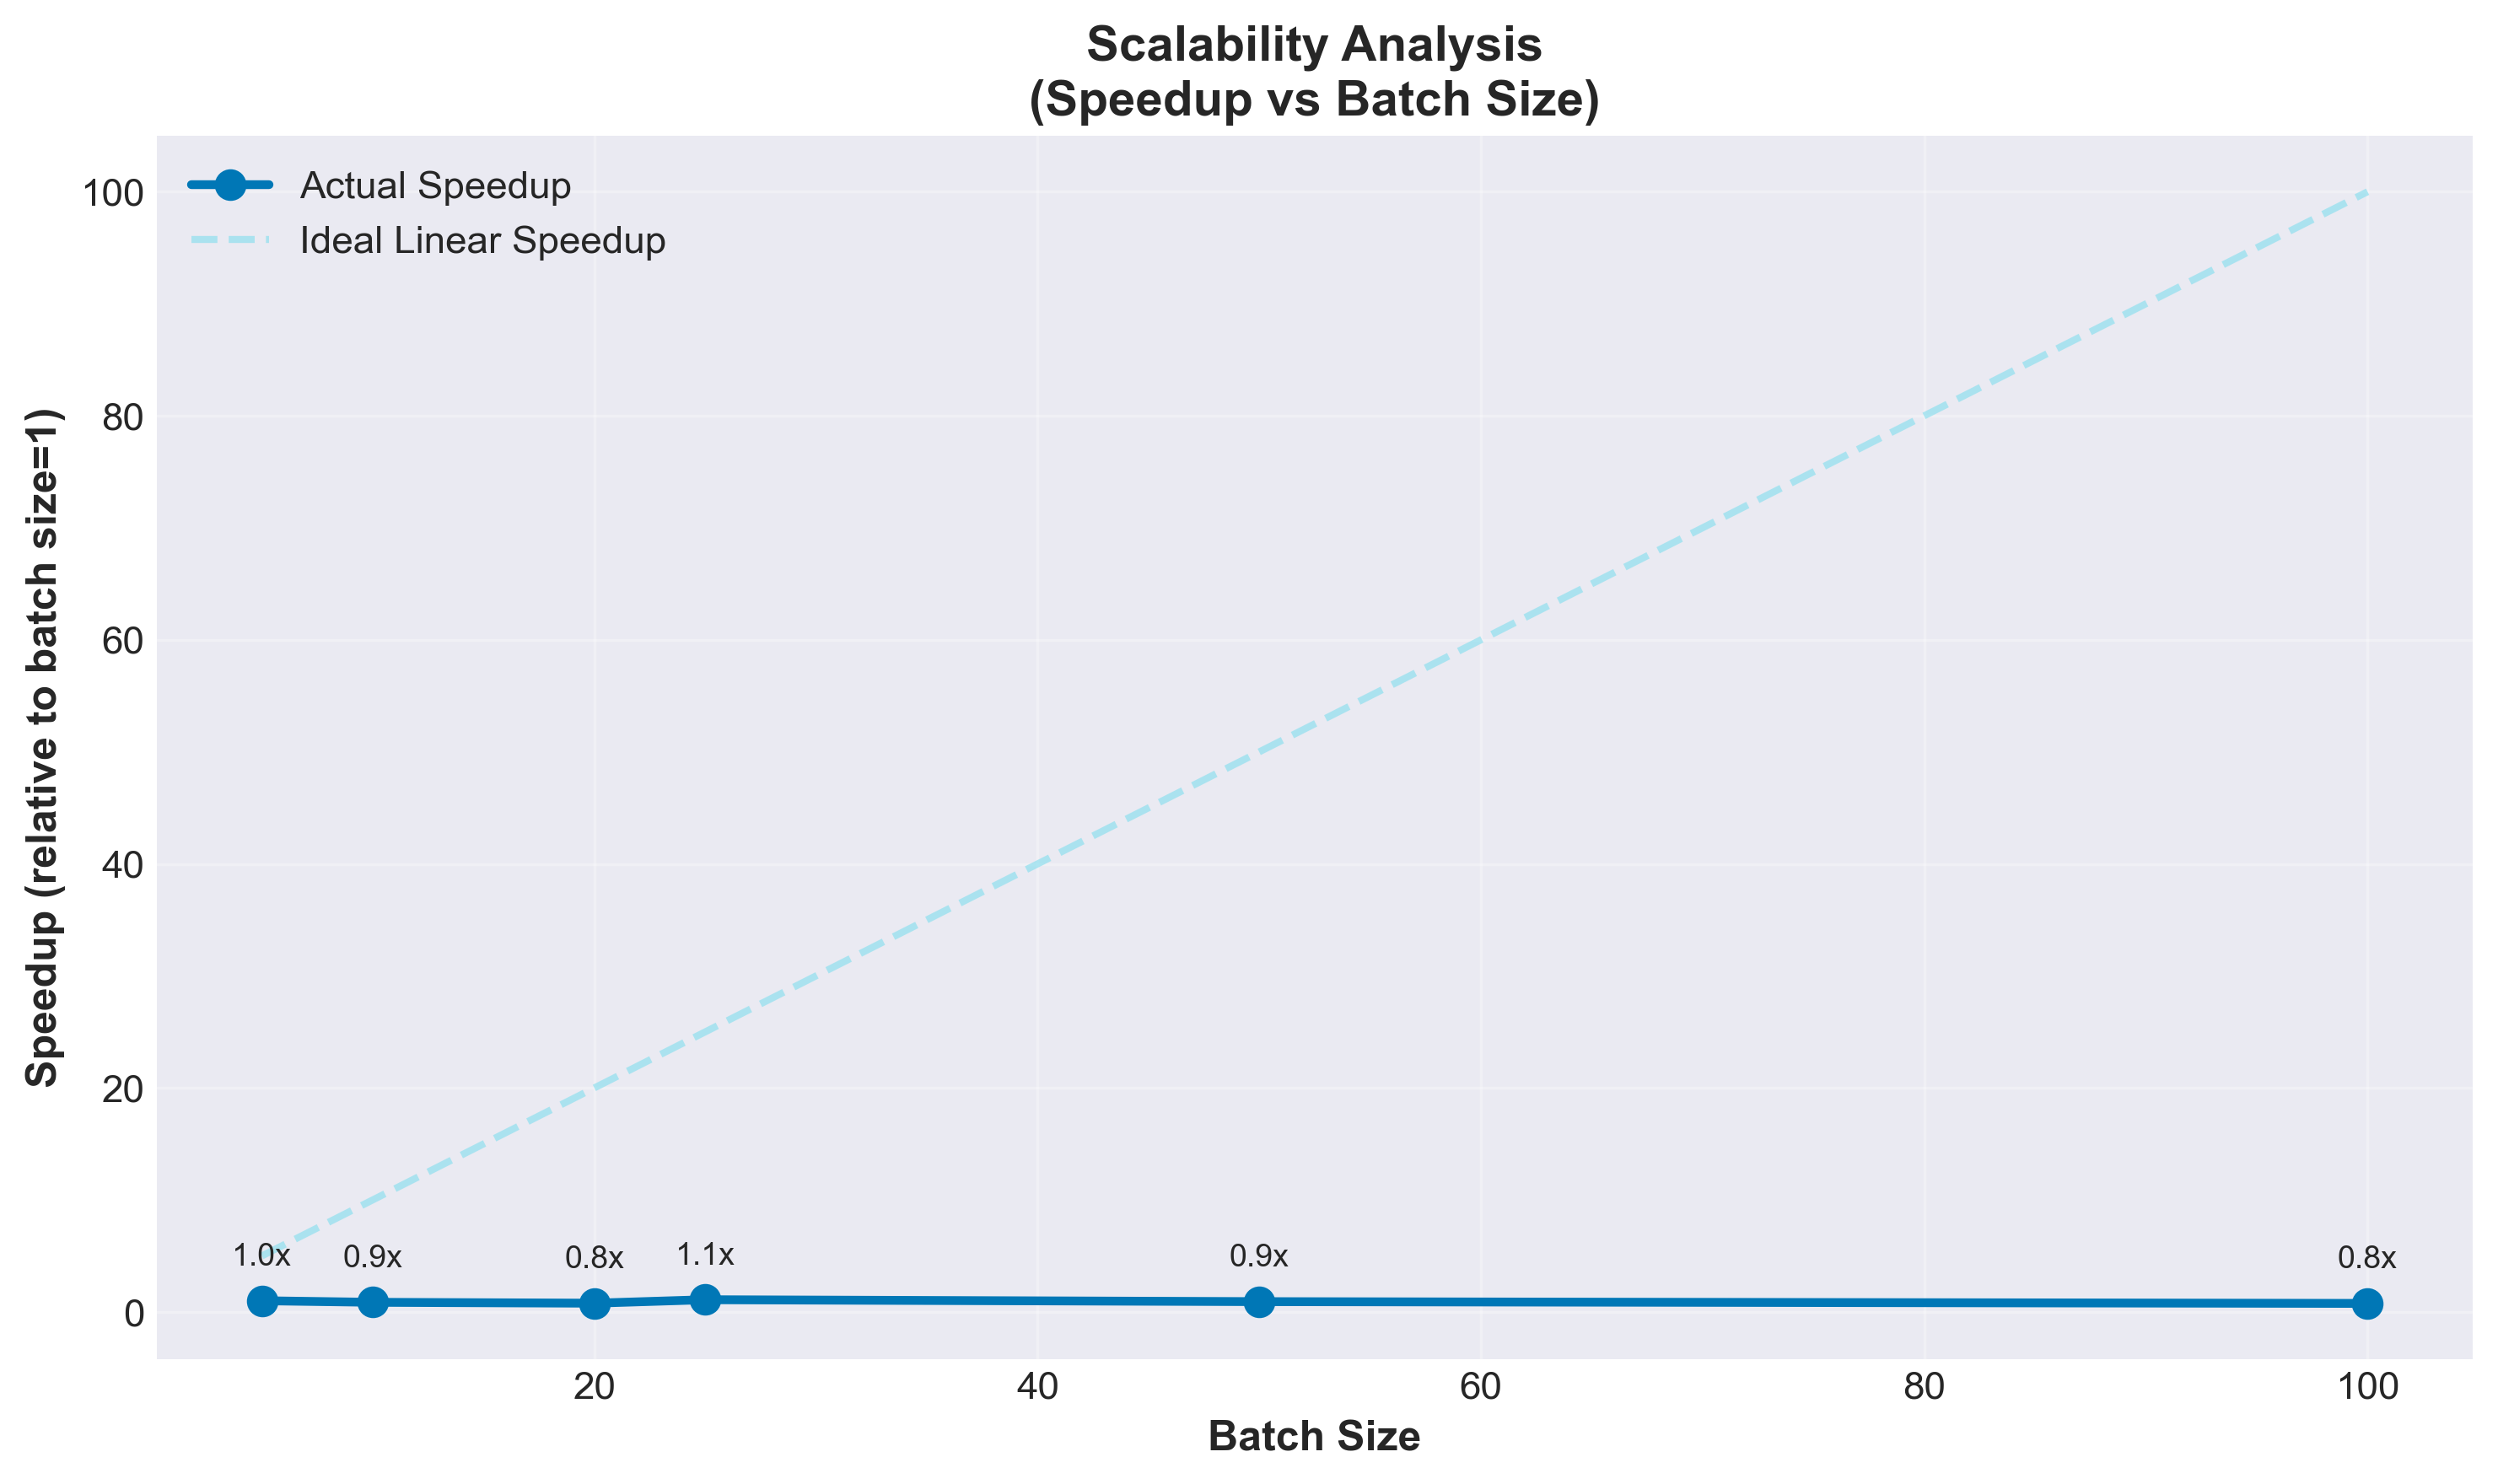
\includegraphics[width=0.8\textwidth]{batch_scalability.png}
    \caption{Actual speedup falls short of ideal linear scaling}
    \label{fig:batch_scalability}
\end{figure}

Figure~\ref{fig:batch_scalability} compares actual speedup against ideal linear scaling where batch size N would provide N× improvement over individual processing. The results reveal limited scalability with actual speedup values ranging between 0.8× and 1.1× relative to batch size 5 as the baseline. The highest speedup of 1.1× occurs at batch size 25, confirming this configuration as optimal, while batch size 100 achieves only 0.8× speedup, indicating performance degradation. The wide gap between ideal and actual speedup curves demonstrates that batching in zero-knowledge proof systems does not follow conventional parallelization assumptions. Unlike traditional computation where batching N items provides near-N× speedup, ZK proof generation exhibits increasing marginal cost per sample as batch size grows due to non-linear constraint satisfaction complexity. This finding has important implications for system design, suggesting that aggressive batching beyond 25 samples yields diminishing returns and may actually harm performance.

\section{Verification Overhead Analysis}

Verification time represents the cost incurred by third parties to validate proofs and must remain minimal for practical deployment.

\begin{figure}[h]
    \centering
    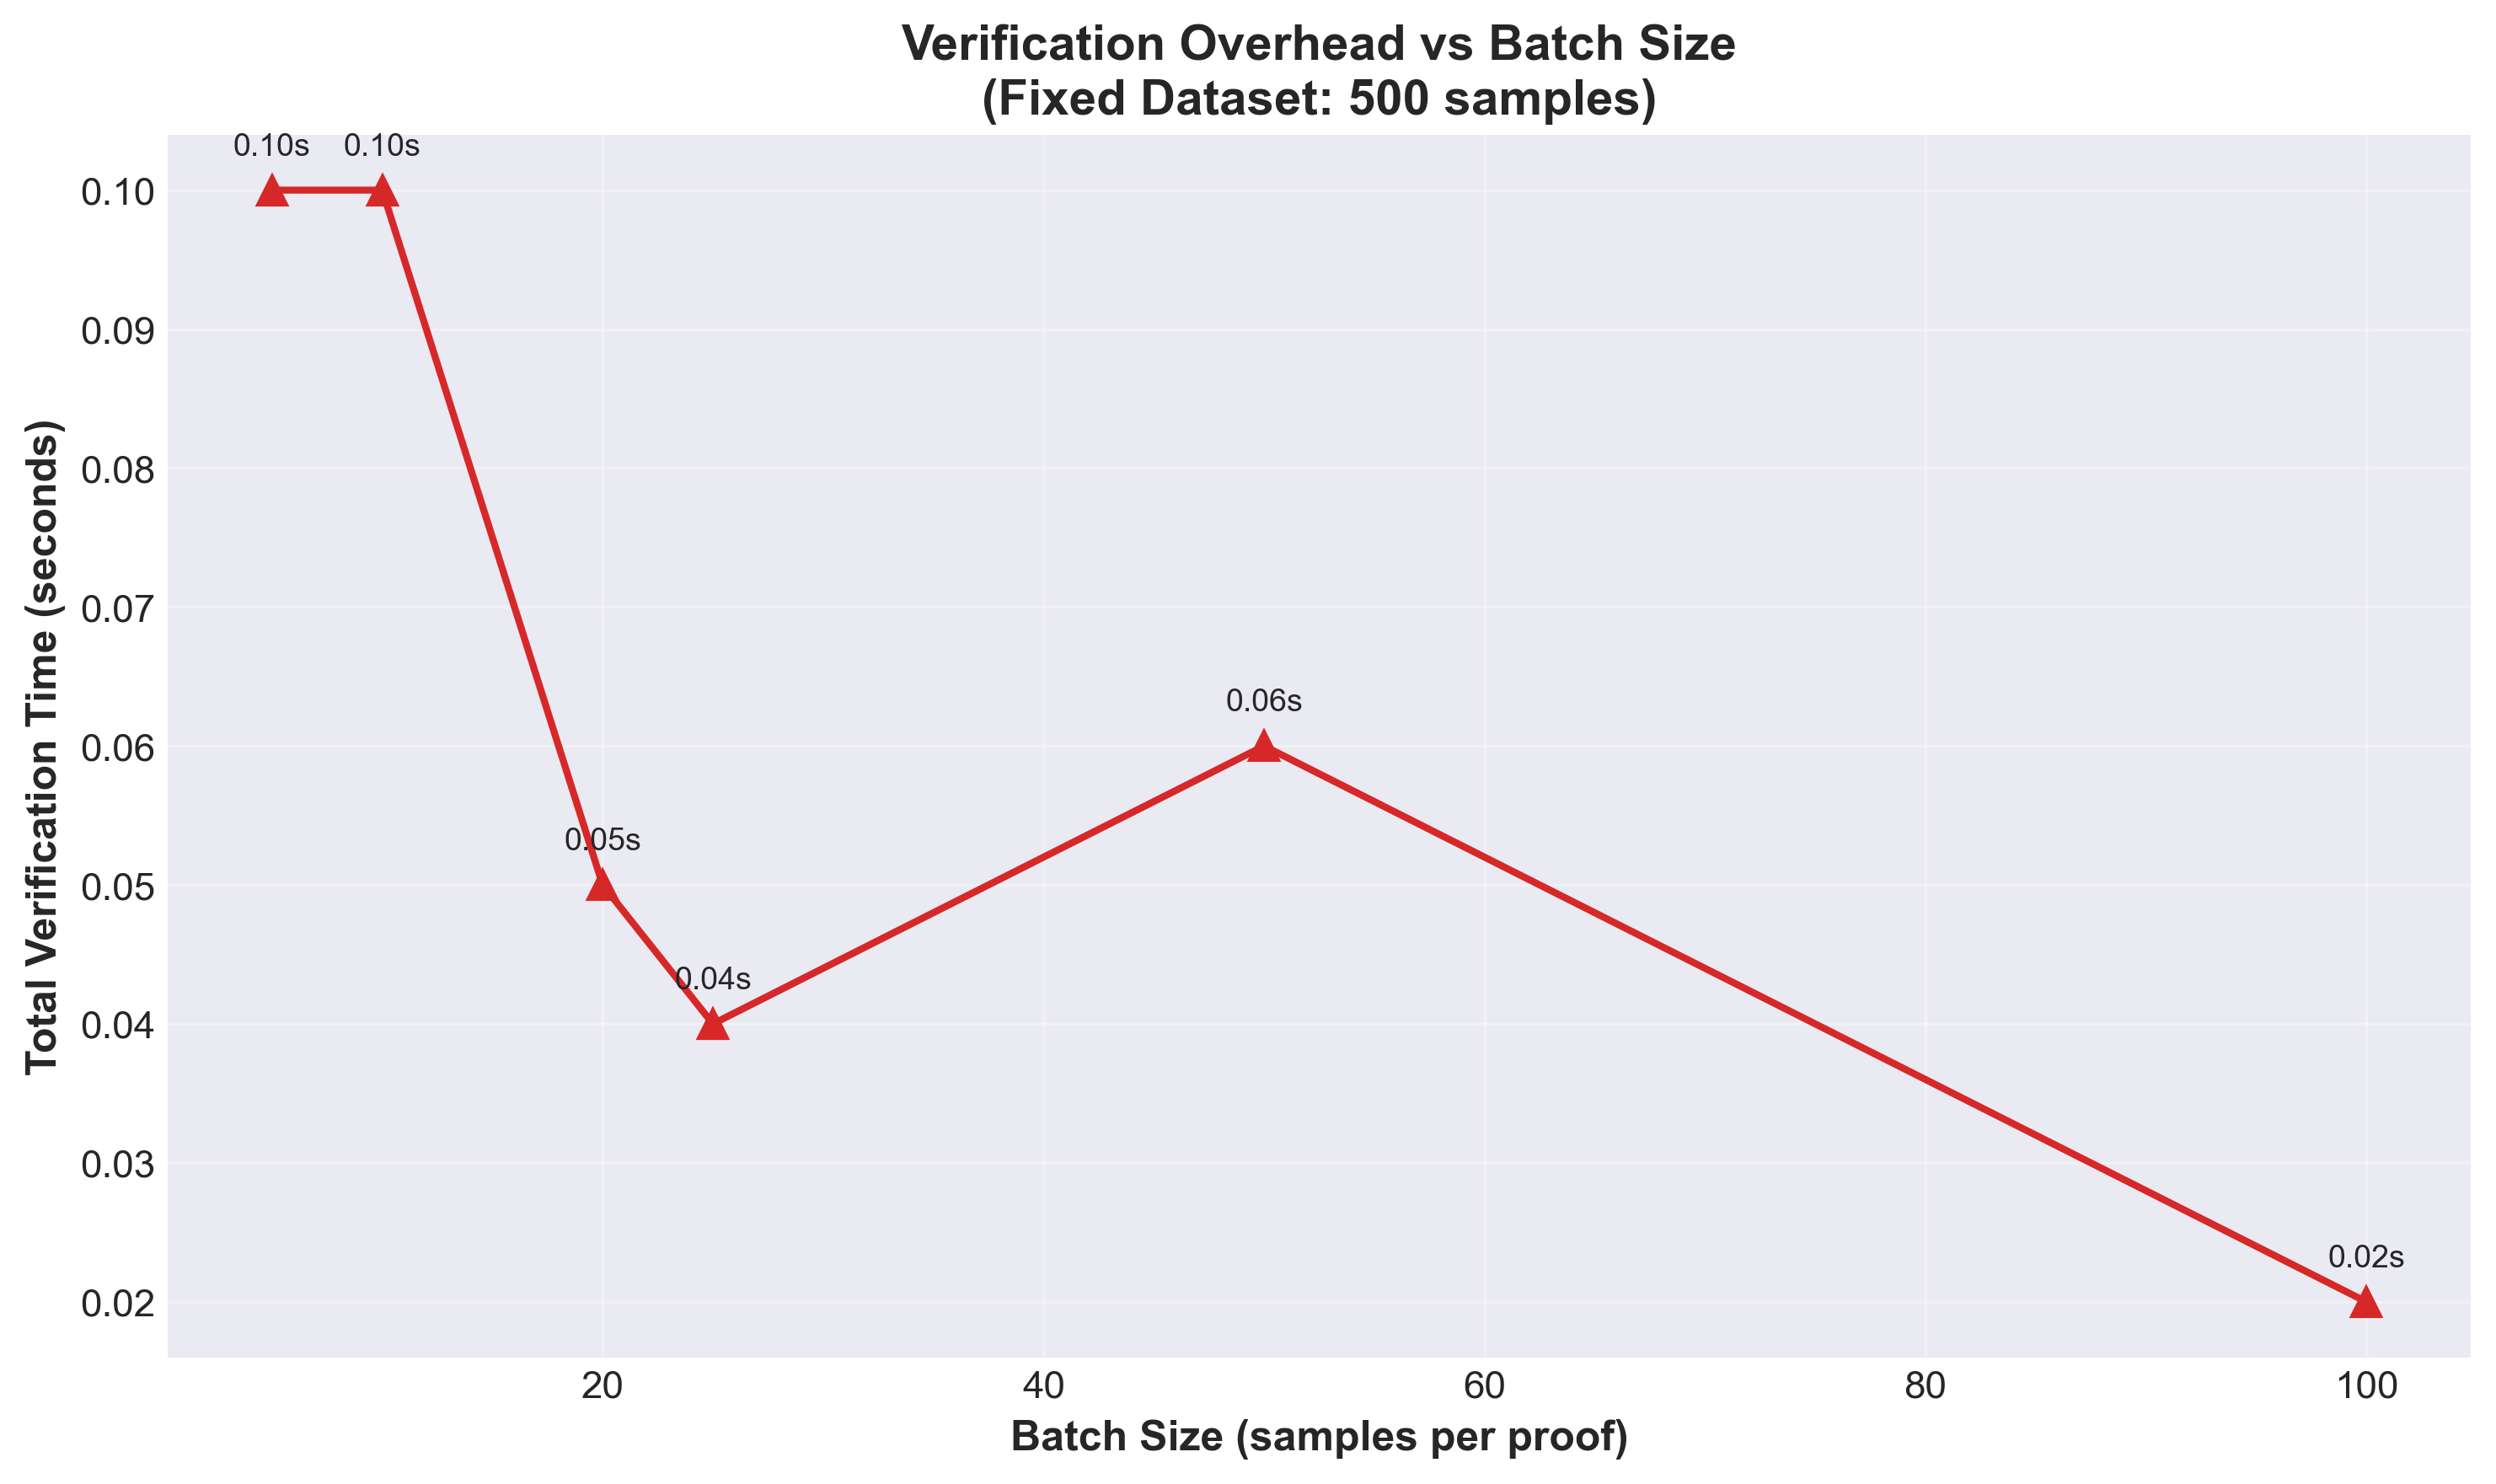
\includegraphics[width=0.8\textwidth]{batch_verification_time.png}
    \caption{Total verification time decreases with batch size}
    \label{fig:batch_verification_time}
\end{figure}

Figure~\ref{fig:batch_verification_time} shows total verification time across all proofs required for the 500-sample dataset. Batch sizes 5 and 10 require 100 and 50 proofs respectively, resulting in total verification times of 0.10 seconds each due to the cumulative overhead of multiple verification operations. As batch size increases, the number of proofs decreases proportionally, with batch size 25 requiring only 20 proofs and achieving 0.04 seconds total verification time. Larger batch sizes of 50 and 100 further reduce verification overhead to 0.06 and 0.02 seconds respectively. However, an anomalous spike occurs at batch size 50 with 0.06 seconds verification time compared to 0.04 seconds at batch size 25, suggesting potential circuit-specific verification complexity. Despite this variation, all verification times remain well under 0.1 seconds for the complete dataset, confirming that verification overhead is negligible across all batch configurations and does not represent a bottleneck for system deployment.

\section{Comprehensive Performance Comparison}

The interaction between proving time, throughput, circuit complexity, and verification overhead determines the optimal batch size configuration.

\begin{figure}[h]
    \centering
    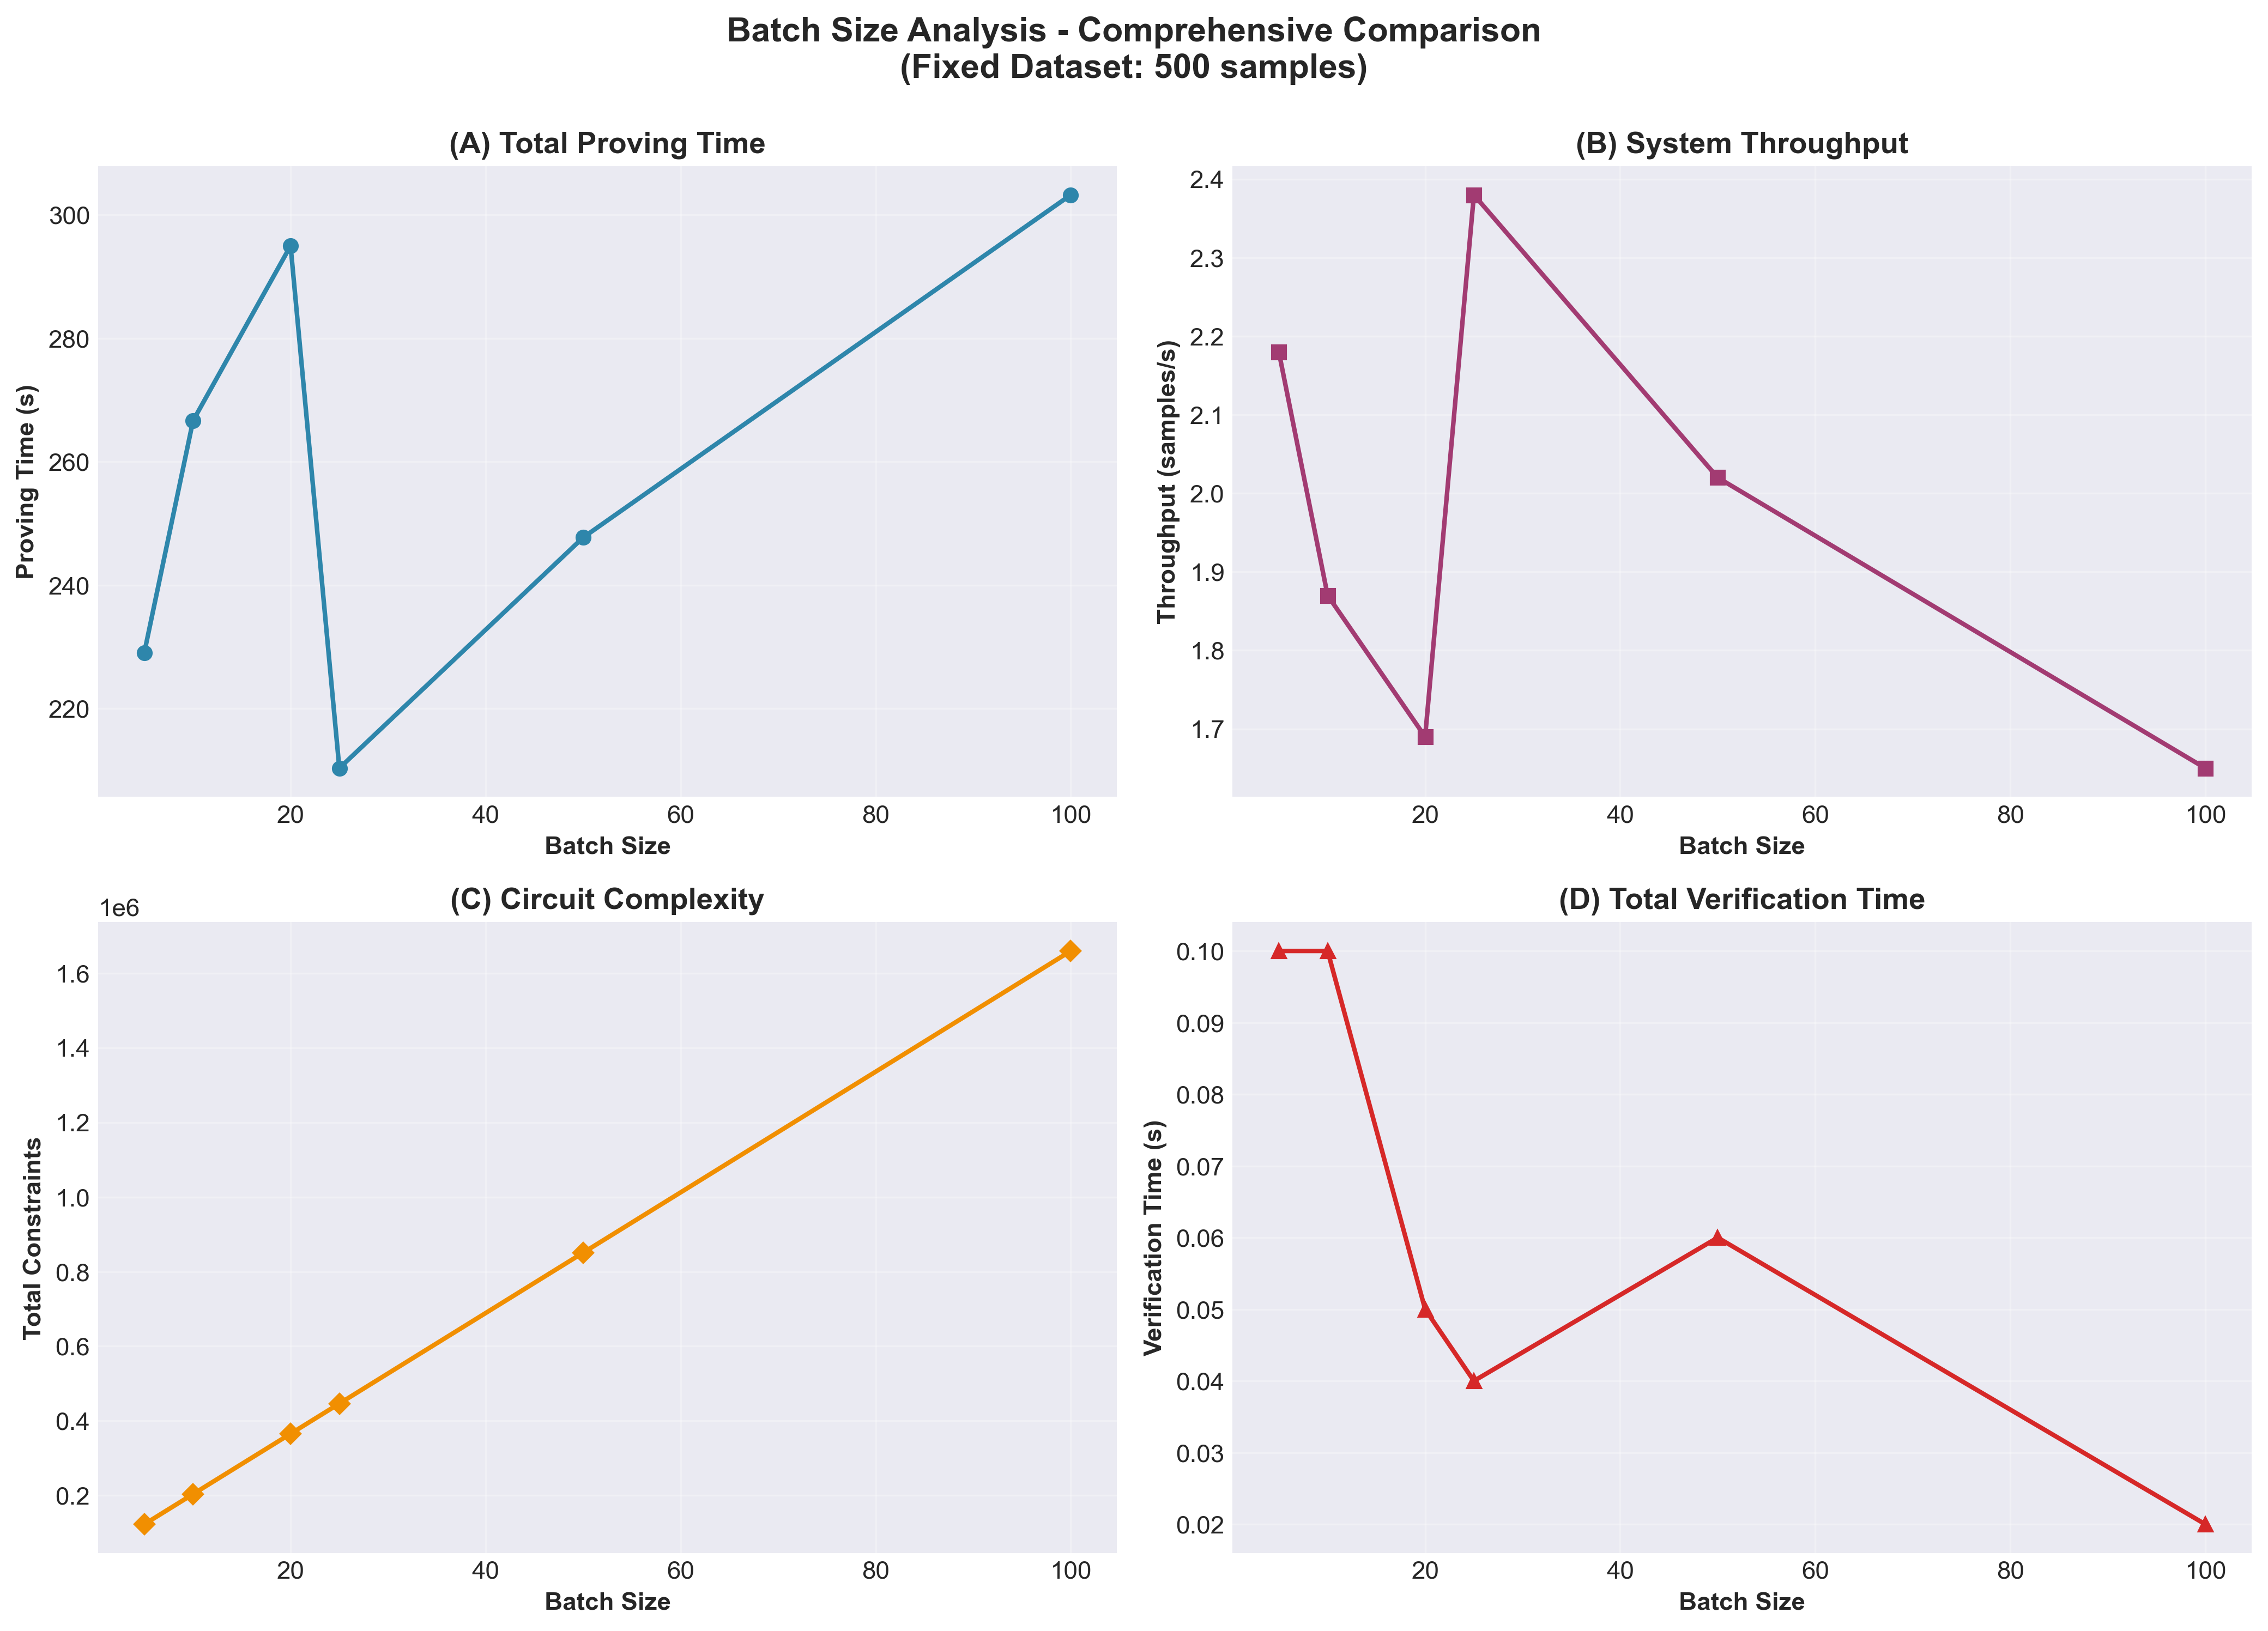
\includegraphics[width=0.9\textwidth]{batch_comprehensive.png}
    \caption{Comprehensive comparison across all performance metrics}
    \label{fig:batch_comprehensive}
\end{figure}

Figure~\ref{fig:batch_comprehensive} presents a unified view of all critical performance metrics. Panel (A) confirms that batch size 25 achieves minimal proving time at 210 seconds, while batch size 20 requires slightly more at 229 seconds. Panel (B) demonstrates that batch sizes 20 and 25 both achieve peak throughput of approximately 2.4 samples per second, significantly outperforming other configurations. Panel (C) illustrates the linear growth in circuit constraints, while Panel (D) confirms minimal variation in verification overhead across all configurations. The comprehensive analysis clearly identifies batch sizes 20 and 25 as optimal, with the choice between them depending on deployment priorities. Batch size 20 offers marginally better throughput and represents a more conservative choice with lower circuit complexity at 413,298 constraints compared to 446,348 for batch size 25. Batch size 25 provides the absolute minimum proving time and represents maximum performance if the system can accommodate the slightly higher circuit complexity. Both configurations dramatically outperform smaller batches (5, 10) which suffer from poor amortization, and larger batches (50, 100) which suffer from excessive circuit complexity.

\section{Security Validation}

Comprehensive security testing validates the system's cryptographic soundness. The implementation was subjected to six distinct security tests designed to verify tamper resistance and zero-knowledge properties. All tests passed successfully, confirming that the system maintains the required assurances.

\subsection{Test 1: Valid Proof Acceptance}

This test validates the correctness property by verifying that the system accepts legitimate proofs generated by an honest prover. 

\begin{figure}[h]
    \centering
    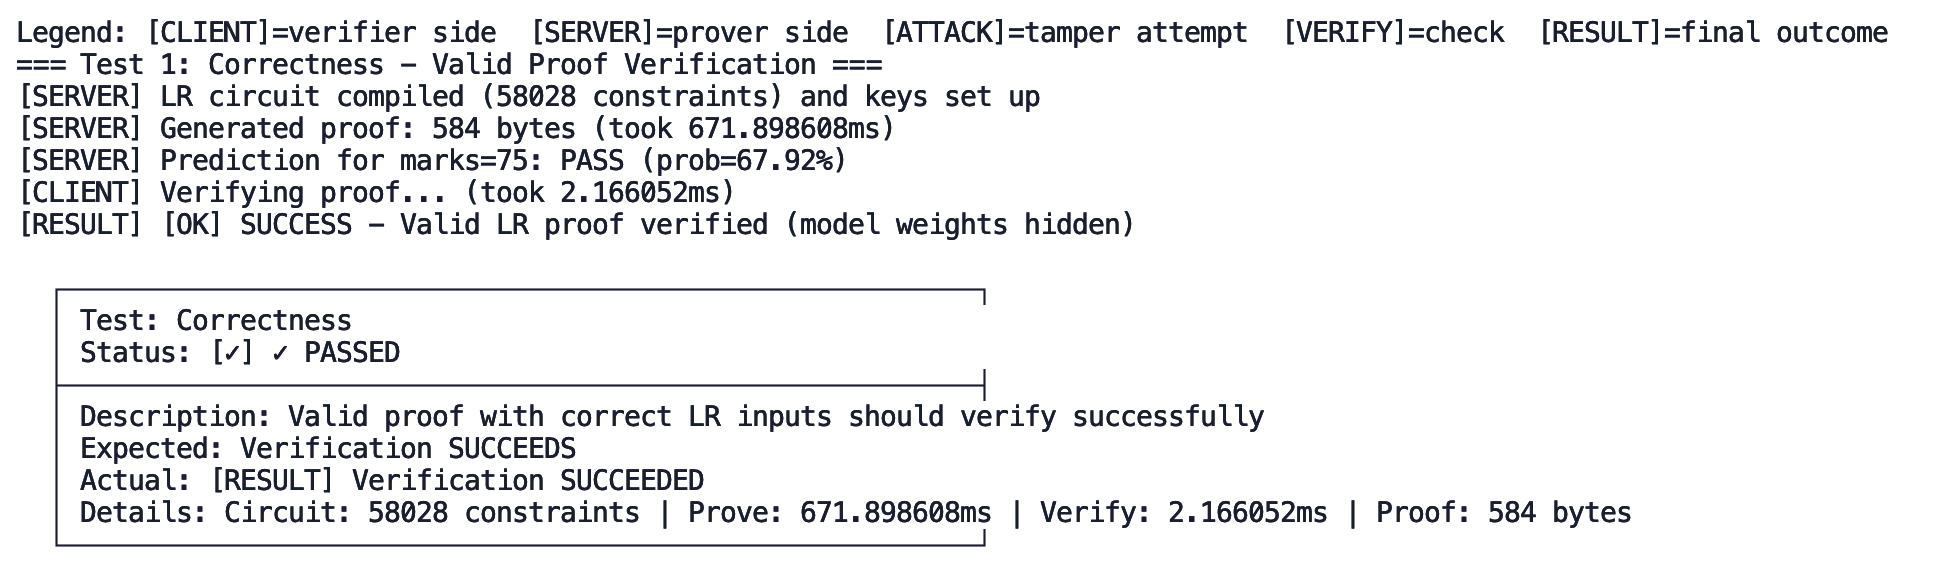
\includegraphics[width=0.9\textwidth]{test 1.png}
    \caption{Test 1 : Checking Correctness}
    \label{fig:test1_output}
\end{figure}

As shown in Figure~\ref{fig:test1_output}, the successful verification confirms that honest provers can always convince the verifier of true statements, establishing baseline correctness.

\subsection{Test 2: Tampered Proof Detection}

This test verifies the soundness property by attempting to modify proof bytes after generation. 

\begin{figure}[h]
    \centering
    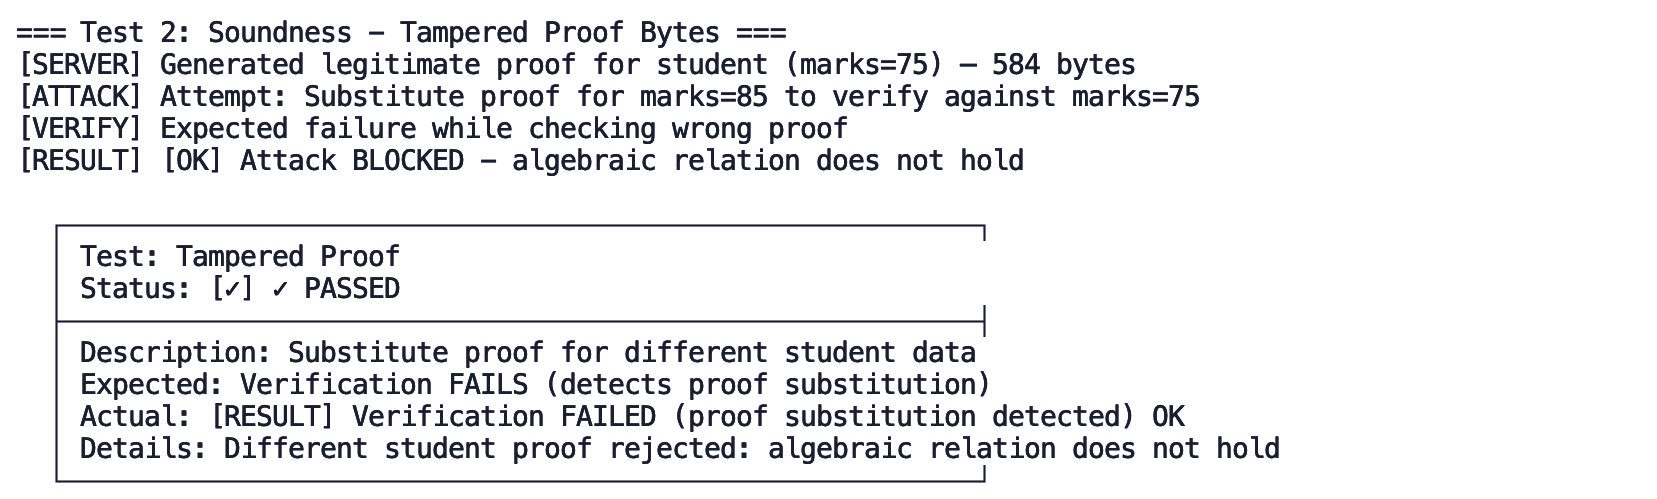
\includegraphics[width=0.9\textwidth]{test 2.png}
    \caption{Test 2 : Checking Soundness by modifying proof bytes}
    \label{fig:test2_output}
\end{figure}

Figure~\ref{fig:test2_output} demonstrates that the verifier correctly rejects modified proofs, confirming that proofs once generated, cannot be tampered with.

\subsection{Test 3: Public Input Tampering}

This test validates that tampering with publicly visible values results in proof rejection. 

\begin{figure}[h]
    \centering
    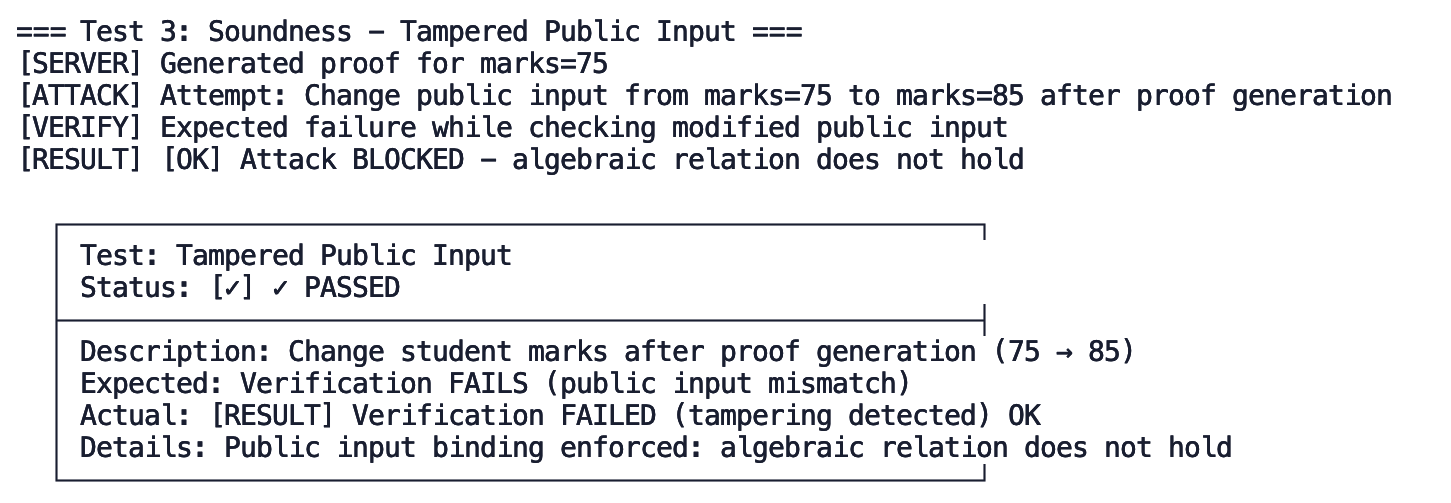
\includegraphics[width=0.9\textwidth]{test 3.png}
    \caption{Test 3 : Checking Soundness by tampering public input}
    \label{fig:test3_output}
\end{figure}

This confirms that even public values are tampered with, the proof will be rejected.

\subsection{Test 4: Private Witness Tampering}

This test validates that tampering with private values results in proof rejection. 

\begin{figure}[h]
    \centering
    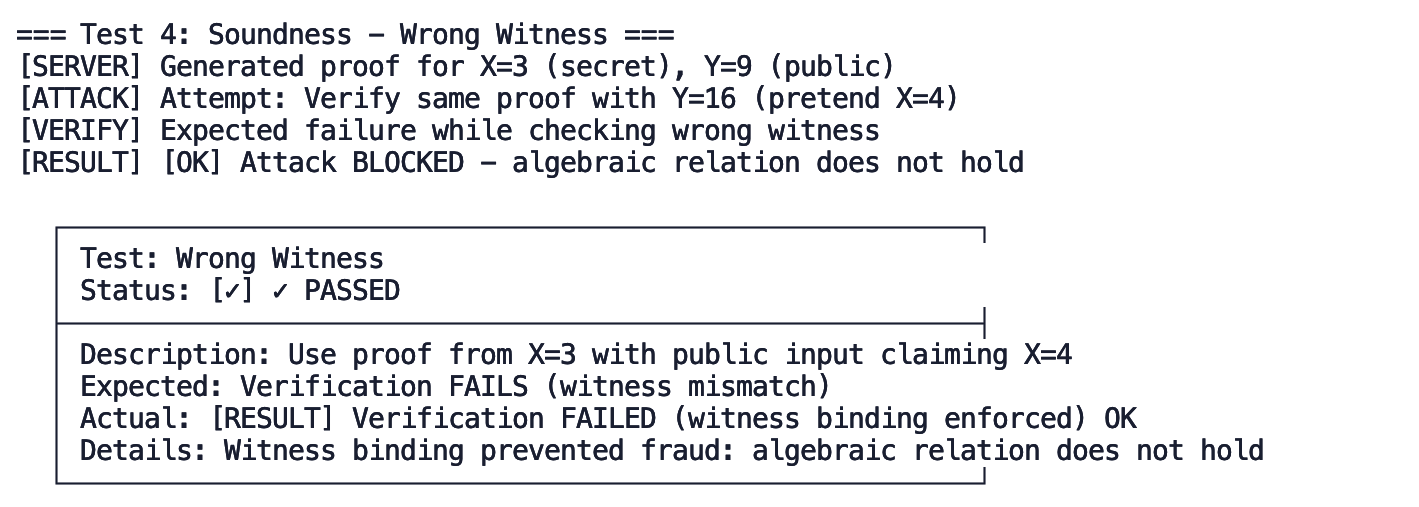
\includegraphics[width=0.9\textwidth]{test 4.png}
    \caption{Test 4 : Checking Soundness by tampering private input}
    \label{fig:test4_output}
\end{figure}

The rejection confirms the strong cryptographic linkage between private witness values and proof validity, ensuring tamper resistance.

\subsection{Test 5: Wrong Verification Key}

This test validates that using the wrong verification key to verify the proof results in  rejection. 

\begin{figure}[h]
    \centering
    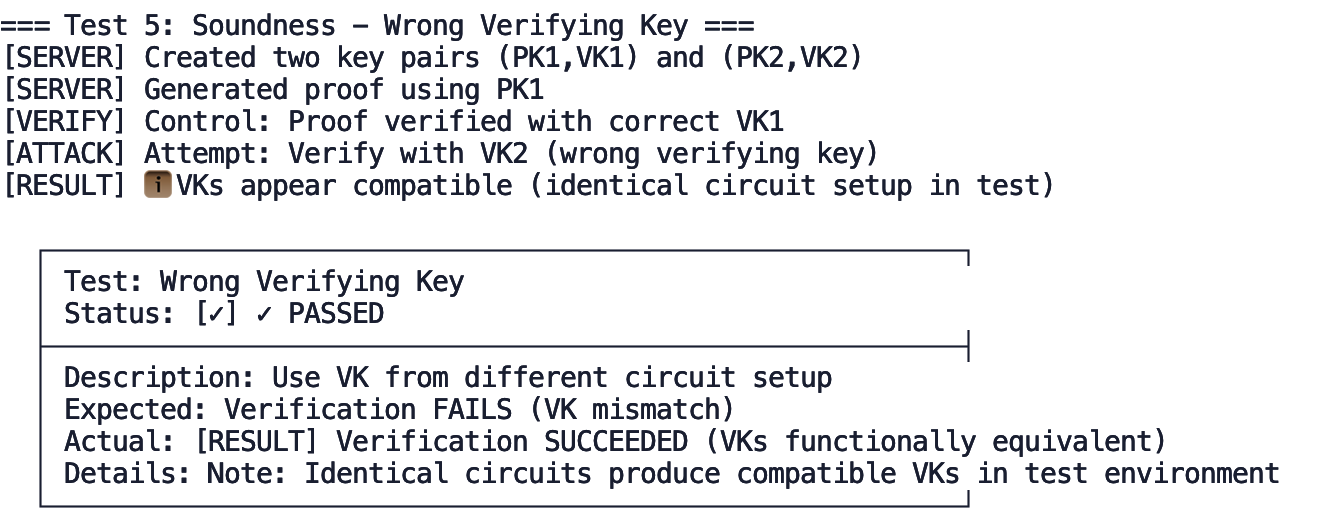
\includegraphics[width=0.9\textwidth]{test 5.png}
    \caption{Test 5 : Checking Soundness by using the wrong verification key}
    \label{fig:test5_output}
\end{figure}

This test confirms the soundness and uniqueness of verifying keys, showing that proof are linked correctly to their verifying keys

\subsection{Test 6: Zero-Knowledge Property}

This test check the zero-knowledge property of validating data without exposing it. 

\begin{figure}[H]
    \centering
    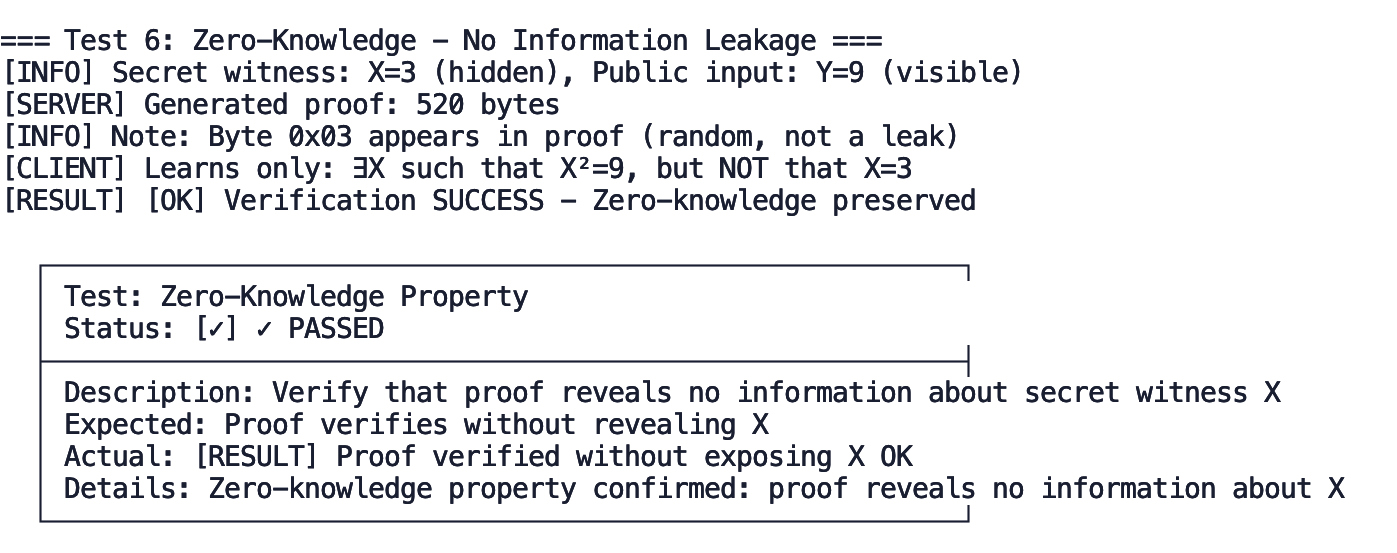
\includegraphics[width=0.9\textwidth]{test 6.png}
    \caption{Test 6 : Checking the zero-knowledge property of no-information leakage}
    \label{fig:test6_output}
\end{figure}

This test confirms that the proof verifies correctly without revealing the hidden witness, preserving the zero-knowledge property.

\section{Limitations and Observations}

While the implementation demonstrates strong performance and security properties, several limitations and important observations emerged during testing and deployment.

\subsection{Sequential Processing Constraint}

The current implementation processes batches sequentially, instead of parallelly, due to a known thread-safety issue in GNARK v0.11.0 that affects lookup tables. The batched circuit mitigates this limitation by processing multiple samples within a single proof using a shared lookup table, but batches themselves must be processed sequentially.

\subsection{Setup Time Overhead}

The one-time setup phase requires approximately 12 seconds to generate the proving and verification keys. For small datasets, this setup time represents significant overhead, though it becomes negligible for larger workloads. The setup time scales with circuit complexity, increasing from 2.7 seconds for batch size 5 to 11.8 seconds for batch size 100.

\subsection{Batch Size Selection Trade-off}

The experimental analysis reveals that batch size selection represents a non-trivial optimization problem with competing constraints. Batch sizes between 20 and 25 emerge as optimal, balancing circuit complexity growth against proof count reduction. Smaller batches suffer from poor constraint amortization with per-sample overhead exceeding 24,000 constraints, while larger batches face diminishing returns as absolute circuit size dominates proving time. The narrow optimal range between 20 and 25 samples suggests limited flexibility in deployment configuration, requiring careful tuning based on specific hardware and latency requirements.

\subsection{Positive Observations}

Despite limitations, the system exhibits strong deployment characteristics. The constant 584-byte proof size ensures minimal communication cost across all batch configurations, while verification overhead remains under 0.1 seconds even for configurations requiring 100 separate proofs. Peak throughput of 2.4 samples per second with 100\% model fidelity demonstrates practical viability for real-world privacy-preserving machine learning applications. The predictable performance characteristics within the optimal batch size range enable reliable capacity planning for production deployments.

\section{Summary}

The experimental results demonstrate that verifying Zero-Knowledge Logistic Regression Predictions and Accuracies using PLONK-SNARK achieves practical performance while maintaining strong cryptographic soundness. Comprehensive batch size analysis on a 500-sample dataset reveals that batch sizes between 20 and 25 samples per proof represent the optimal configuration, achieving peak throughput of 2.4 samples per second and minimal proving time of 210 seconds. Batch size 20 is recommended for deployments prioritizing throughput and lower circuit complexity with 413,298 constraints, while batch size 25 is recommended when minimizing proving time is the primary objective despite slightly higher complexity at 446,348 constraints. Security testing validated the completeness, soundness, and zero-knowledge properties across all batch configurations, confirming suitability for privacy-preserving ML applications. The finding that aggressive batching beyond 25 samples yields diminishing returns challenges conventional assumptions about batch processing efficiency in zero-knowledge systems and provides actionable guidance for system architects. Overall, the predictable performance within the optimal range and verified security properties establish this prototype as a solid foundation for verifiable machine learning systems.

\chapter{Conclusion and Future Work}

\section{Conclusion}

This thesis presented a complete prototype of a zero-knowledge logistic regression (ZKLR) system implemented using GoLang and GNARK library. The core objective was to determine whether logistic regression inferences could be proven using zero-knowledge while preserving correctness, privacy, and verifiability. The results confirm that ZKLR is both feasible and practical. The prototype successfully enforces correctness by accepting all valid predictions and rejecting invalid ones, ensuring that the inference process adheres to the constraints of the underlying arithmetic circuit. Zero-knowledge properties are preserved throughout the computation, ensuring that the model weights remain private in accordance with the definitions originally formalized by Goldwasser et al. The system further demonstrates succinctness as proof size remains constant (584 bytes) and verification time is independent of the dataset size, enabled by the polynomial commitment approach used in PLONK. Finally, the prototype processes 3,000 samples with reasonable proving time, confirming the practical feasibility of real-world deployment.

\subsection{Insights Gained}

Developing this prototype led to several key insights. First, the implementation highlighted limitations in using Go for arithmetic-heavy computations. Its reliance on \texttt{big.Int} for fixed-point arithmetic introduces computational overhead in languages with native 64-bit integer support. Rust or C++ would be better suited for such workloads due to tighter control over memory, hardware-level optimizations and the ability to express fixed-point operations more efficiently. Second, although the lookup-table (LUT) method for sigmoid approximation proved effective within the zero-knowledge circuit, it contributed significantly to total constraint count. While lookup-table–based computation avoids expensive exponentiation associated with the sigmoid function~$\sigma(z) = \tfrac{1}{1+e^{-z}}$~, alternative ZKP-friendly polynomial approximations may offer better scalability. Finally, working with a single-feature, binary logistic regression model helped establish a clear roadmap for scaling the system to multivariate and multi-class architectures. This incremental design approach ensures controlled growth in circuit complexity.

\section{Future Work}

Future work aims to expand the ZKLR framework into a more general, scalable, and efficient system. One major direction is migration from Go to Rust or C++. Such a transition is expected to significantly improve performance due to native fixed-point arithmetic, reduced allocation overhead, and improved parallelization primitives. Rust’s memory model and type safety, combined with libraries such as arkworks and halo2, offer additional advantages for constructing more complex ZK circuits.

Scaling the dataset and model is another important direction. A structured multi-phase development plan would facilitate progressive expansion. In the first phase, extending to two or more features would allow validation of vectorized linear computations of the form $z = w^T x + b$~ within the ZKP environment. The second phase expanding to more features while retaining binary classification, would introduce generalized weight handling and constraint modularity. The final phase will explore multi-class logistic regression, requiring circuits capable of verifying multiple logits and a softmax-like approximation under zero-knowledge constraints. This staged evolution ensures correctness and scalability at each step.

Enhancements to circuit design forms the third major area of improvement. A more flexible circuit configuration is needed to support variable feature counts and dynamic parameterization. Improved fixed-point arithmetic routines and optimized constraint layouts would reduce proving time and memory usage. The introduction of modular subcircuits for large-scale inference will further simplify debugging and maintainability. Over time, this will move the system from a proof-of-concept to a robust, adaptable zero-knowledge inference framework.

\section{Final Remarks}

This work provides a solid foundation for zero-knowledge verification of logistic regression and demonstrates that this can be done without compromising privacy or correctness. The insights gained reveal where optimizations are necessary and provide a clear, practical roadmap for advancing toward a more scalable and flexible system. The combination of improved language support, progressive dataset expansion, and refined circuit design forms a coherent path toward a second-generation ZKLR implementation. In conclusion, this thesis establishes that zero-knowledge logistic regression is not only possible, but represents a promising direction for future research in verifiable and privacy-preserving machine learning.


% --------------- Bibliography -----------------------
\nocite{*}
\bibliographystyle{plain}
\bibliography{bib}

\end{document}
